% Using fithesis2 LaTeX style.
% Required files: fithesis2.cls, fit12.clo, fi-logo.mf

% fithesis2 home page:
% http://is.muni.cz/th/173173/fi_b/?info

% fithesis2 documentation:
% http://is.muni.cz/th/173173/fi_b/thesis.pdf?info

% fithesis2 download:
% http://is.muni.cz/th/173173/fi_b/fithesis2.zip?info

%\documentclass[draft]{fithesis2} % Default: [12pt,oneside,onecolumn,final]
\documentclass{fithesis2} % Default: [12pt,oneside,onecolumn,final]
\usepackage{bachelor}
%%
%% This is file `fithesis2.cls',
%% it's a software fork based on class fithesis v0.2.11 available
%% to download from http://www.fi.muni.cz/~xpavlov/fithesis/
%% This file is distributed under LPPL Version 1.3c

\NeedsTeXFormat{LaTeX2e}
\ProvidesClass{fithesis2}[2008/12/15 version 0.1 MU thesis class]

\ifx\clsclass\undefined
 \def\clsclass{rapport3}
\fi
\LoadClass{\clsclass}

% Declaration of documentclass options 
\DeclareOption{10pt}{\renewcommand\@ptsize{0}}
\DeclareOption{11pt}{\renewcommand\@ptsize{1}}
\DeclareOption{12pt}{\renewcommand\@ptsize{2}}
\DeclareOption{oneside}{\@twosidefalse \@mparswitchfalse}
\DeclareOption{twoside}{\@twosidetrue  \@mparswitchtrue}
\DeclareOption{onecolumn}{\@twolumnfalse}
\DeclareOption{twocolumn}{\@twocolumntrue}
\DeclareOption{draft}{\setlength\overfullrule{5pt}}
\DeclareOption{final}{\setlength\overfullrule{0pt}}

% Options executed by default
\ExecuteOptions{12pt,oneside,final}
\ProcessOptions

\RequirePackage{palatino}

\def\Scrreprtcls{scrreprt}
\def\Rapport1cls{rapport1}
\def\Rapport3cls{rapport3}

\ifx\clsclass\Scrreprtcls
 \newcommand*\ChapFont{\bfseries}
 \newcommand*\PageFont{\bfseries}
\fi

% depth of table of content (TOC)
% TOC will contain sectioning commands upto \subsubsection
\setcounter{tocdepth}{4}

% loads fit1*.clo size option class
\input fit1\@ptsize.clo\relax

\def\ps@thesisheadings{%
\def\chaptermark##1{%
\markright{%
\ifnum\c@secnumdepth >\m@ne
\thechapter.\ %
\fi ##1}}
\let\@oddfoot\@empty
\let\@oddhead\@empty
\def\@oddhead{\vbox{\hbox to \textwidth{%
\hfil{\sc\rightmark}}\vskip 4pt\hrule}}
\if@twoside
 \def\@evenhead{\vbox{\hbox to \textwidth{%
 {\sc\rightmark}\hfil}\vskip 4pt\hrule}}
\else
 \let\@evenhead\@oddhead
\fi
\def\@oddfoot{\hfil\PageFont\thepage}
\if@twoside
 \def\@evenfoot{\PageFont\thepage\hfil}%
\else
 \let\@evenfoot\@oddfoot
\fi
}

% defines style of the chapter heading
\renewcommand*\chapter{%
\if@twoside
 \clearpage
 \thispagestyle{empty}
 \cleardoublepage
\else
 \clearpage
\fi
\thispagestyle{plain}%
\global\@topnum\z@
\@afterindentfalse
\secdef\@chapter\@schapter}

% defines style of part heading
\renewcommand*\part{%
\clearpage
\thispagestyle{empty}
\cleardoublepage
\thispagestyle{empty}%
\if@twocolumn%
 \onecolumn
 \@tempswatrue
\else
 \@tempswafalse
\fi
\hbox{}\vfil
\secdef\@part\@spart}

% defines commands to typeset logos and default names of university,
% faculty and thesis title on the title page
\font\filogo fi-logo at 40mm % as logo of FI, METAFONT logo will be used
\def\facultylogo{\@thesisfaculty-logo} % log format
\def\universityname{Masarykova univerzita} % default university name
\def\facultyname{Fakulta informatiky} % default faculty name
\def\@thesissubtitle{Diplomov\'{a} pr\'{a}ce} % default thesis title
\def\lowecasewrapper#1{\lowercase{#1}}

% definition of \thesisfaculty options 
\def\Fi{fi} % Faculty of Informatics
\def\Sci{sci} % Faculty of Science
\def\Law{law} % Faculty of Law
\def\Eco{eco} % Faculty of Economics and Administration
\def\Fss{fss} % Faculty of Social studies
\def\Med{med} % Faculty of Medicine
\def\Ped{ped} % Faculty of Education
\def\Phil{phil} % Faculty of Arts
\def\Fsps{fsps} % Faculty of Sport Studies
\def\True{true}

% definition of language support: Czech (default), English and Slovak
\def\Langcs{cs}
\def\Langsk{sk}
\def\Langen{en}
\def\@thesislang{cs}

% definition of commands that will be used to typeset title page
% can be redefined in the source document
\def\titlefont{\fontsize\@xxvpt{30}\selectfont} 
\def\thesistitle#1{\gdef\@thesistitle{#1}}
\def\thesisstudent#1{\gdef\@thesisstudent{#1}}
\def\thesisyear#1{\gdef\@thesisyear{#1}}
\def\thesisplaceyear{Brno, \@thesisyear}
\def\thesissubtitle#1{\gdef\@thesissubtitle{#1}}
\def\thesisuniversity#1{\gdef\@thesisuniversity{#1}}
\def\thesislogo#1{\gdef\@thesislogo{#1}}
\def\thesisadvisor#1{\gdef\@thesisadvisor{#1}}
% option of \thesisfaculty macro defines which name of faculty will be printed
% language option defines whether english or czech name will be used
\def\thesisfaculty#1{\gdef\@thesisfaculty{#1}
\ifx\@thesisfaculty\Fi
 \ifx\@thesislang\Langen
  \def\facultyname{Faculty of Informatics}
  \def\universityname{Masaryk University}
   \else \def\facultyname{Fakulta informatiky}
  \fi
 \else \ifx\@thesisfaculty\Sci
  \ifx\@thesislang\Langen
   \def\facultyname{Faculty of Science}
   \def\universityname{Masaryk University}
  \else \def\facultyname{P\v{r}\'{i}rodov\v{e}deck\'{a} fakulta}
  \fi
  \else \ifx\@thesisfaculty\Law
   \ifx\@thesislang\Langen
    \def\facultyname{Faculty of Law}
    \def\universityname{Masaryk University}
   \else \def\facultyname{Pr\'{a}vnick\'{a} fakulta}
   \fi
  \else \ifx\@thesisfaculty\Eco
   \ifx\@thesislang\Langen
    \def\facultyname{Faculty of Economics and Administration}
    \def\universityname{Masaryk University}
   \else \def\facultyname{Ekonomicko-spr\'{a}vn\'{i} fakulta}
   \fi
  \else \ifx\@thesisfaculty\Fss
   \ifx\@thesislang\Langen
    \def\facultyname{Faculty of Social Studies}
    \def\universityname{Masaryk University}
   \else \def\facultyname{Fakulta soci\'{a}ln\'{i}ch studi\'{i}}
   \fi
  \else \ifx\@thesisfaculty\Med
   \ifx\@thesislang\Langen
    \def\facultyname{Faculty of Medicine}
    \def\universityname{Masaryk University}
   \else \def\facultyname{L\'{e}ka\v{r}sk\'{a} fakulta}
   \fi
  \else \ifx\@thesisfaculty\Ped
   \ifx\@thesislang\Langen
    \def\facultyname{Faculty of Education}
    \def\universityname{Masaryk University}
   \else \def\facultyname{Pedagogick\'{a} fakulta}
   \fi
  \else \ifx\@thesisfaculty\Phil
   \ifx\@thesislang\Langen
    \def\facultyname{Faculty of Arts}
    \def\universityname{Masaryk University}
   \else \def\facultyname{Filozofick\'{a} fakulta}
   \fi
  \else \ifx\@thesisfaculty\Fsps
   \ifx\@thesislang\Langen
    \def\facultyname{Faculty of Sports Studies}
    \def\universityname{Masaryk University}
   \else \def\facultyname{Fakulta sportovn\'{i}ch studi\'{i}}
   \fi
         \else
          \def\facultyname{\@thesisfaculty}
          \def\universityname{\@thesisuniversity}
          \def\facultylogo{\@thesislogo}
          \def\thesisplaceyear{\@thesisyear}
         \fi
        \fi
       \fi
      \fi
     \fi
    \fi
   \fi
  \fi
\fi
}

\newif\if@restonecol

\def\alwayssingle{%
\@restonecolfalse\if@twocolumn\@restonecoltrue\onecolumn\fi}
\def\endalwayssingle{\if@restonecol\twocolumn\fi}

% if the true value is set in the \thesiswoman command
% then character 'a' will be added after verbs in czech and
% slovak language when typesetting declaration text
\newif\ifwoman\womanfalse
\def\@w{\ifwoman{a}\else\fi}
\def\thesiswoman#1{\gdef\@thesiswoman{#1}
\ifx\@thesiswoman\True\def\@w{a}\else\def\@w{}\fi}

\def\thesislang#1{\gdef\@thesislang{#1}}

% Text of Declaration in Czech
\def\DeclarationTextcs{%
Prohla\v{s}uji, \v{z}e tato \expandafter\lowecasewrapper\@thesissubtitle{}
je m\'{y}m p\r{u}vodn\'{i}m autorsk\'{y}m
d\'{i}lem, kter\'{e} jsem vypracoval\@w\ samostatn\v{e}. V\v{s}echny zdroje, prameny a
literaturu, kter\'{e} jsem p\v{r}i vypracov\'{a}n\'{i} pou\v{z}\'{i}val\@w\ nebo z~nich
\v{c}erpal\@w, v~pr\'{a}ci \v{r}\'{a}dn\v{e} cituji s~uveden\'{i}m \'{u}pln\'{e}ho odkazu na p\v{r}\'{i}slu\v{s}n\'{y}
zdroj.}
% in Slovak
\def\DeclarationTextsk{%
Prehlasujem, \v{z}e t\'{a}to \expandafter\lowecasewrapper\@thesissubtitle{}
je moj\'{i}m p\^{o}vodn\'{y}m autorsk\'{y}m
dielom, ktor\'{e} som vypracoval\@w\ samostatne. V\v{s}etky zdroje, pramene a
literat\'{u}ru, ktor\'{e} som pri vypracovan\'{i} pou\v{z}\'{i}val\@w\ alebo z~nich
\v{c}erpal\@w, v~pr\'{a}ci riadne citujem s~uveden\'{i}m \'{u}pln\'{e}ho odkazu na pr\'{i}slu\v{s}n\'{y}
zdroj.}
% in English
\def\DeclarationTexten{%
Hereby I declare, that this paper is my original authorial work,
which I have worked out by my own. All sources, references and literature used or excerpted
during elaboration of this work are properly cited and listed in complete reference to the due source.
}

% Declaration heading in Czech
\def\DeclarationTitlecs{%
Prohl\'{a}\v{s}en\'{i}
}
% in Slovak
\def\DeclarationTitlesk{%
Prehl\'{a}senie
}
% in English
\def\DeclarationTitleen{%
Declaration
}
% Heading of thesis thank
\def\ThanksTitlecs{%
Pod\v{e}kov\'{a}n\'{i}
}

\def\ThanksTitlesk{%
Po\v{d}akovanie
}

\def\ThanksTitleen{%
Acknowledgement
}
% definition of heading of thesis abstract
\def\AbstractTitlecs{%
Shrnut\'{i}
}

\def\AbstractTitlesk{%
Zhrnutie
}

\def\AbstractTitleen{%
Abstract
}

% definiton of heding of thesis Keywords
\def\KeyWordsTitlecs{%
Kl\'{i}\v{c}ov\'{a} slova
}

\def\KeyWordsTitlesk{%
K\v{l}\'{u}\v{c}ov\'{e} slov\'{a}
}

\def\KeyWordsTitleen{%
Keywords
}
% Definition of command used to declare thesis advisor heading
\def\AdvisorTitlecs{%
Vedouc\'{i} pr\'{a}ce:
}

\def\AdvisorTitlesk{%
Ved\'{u}ci pr\'{a}ce:
}

\def\AdvisorTitleen{%
Advisor:
}

% command prints declaration text in defined language
% with name of student under it
\def\DeclarationText{%
\ifx\@thesislang\Langcs
 \DeclarationTextcs
 \else \ifx\@thesislang\Langsk
  \DeclarationTextsk
  \else \ifx\@thesislang\Langen
   \DeclarationTexten
   \else \DeclarationTextcs
  \fi
 \fi
\fi
\vskip 2cm
\hfill\@thesisstudent
}
% prints "Advisor:" in defined language
\def\AdvisorName{\par\vfill{
\ifx\@thesislang\Langcs
 \bf \AdvisorTitlecs
 \else \ifx\@thesislang\Langsk
  \bf \AdvisorTitlesk
  \else \ifx\@thesislang\Langen
   \bf \AdvisorTitleen
   \else \bf \AdvisorTitlecs
  \fi
 \fi
\fi} \@thesisadvisor}

% this command begins compulsory part of the thesis
% page numbering will be roman
\def\FrontMatter{%
\pagestyle{plain}
\parindent 1.5em
\setcounter{page}{1}
\pagenumbering{roman}}

% command to typeset thesis title page
\newcommand{\ThesisTitlePage}{
\begin{alwayssingle}
\thispagestyle{empty}
\begin{center}
{\sc \universityname\\ \facultyname}
\vskip 1em

% if FI then logo in METAFONT format will be typeset
\ifx\@thesisfaculty\Fi
 {\filogo SL}\\[0.4in]
% else logo defined in \facultylogo command will be used
\else
 \includegraphics[width=40mm]{\facultylogo}\\[0.4in]
\fi

% typesets thesis subtitle and the name of author
% with year and place of university
\let\footnotesize\small
\let\footnoterule\relax{}
{\titlefont\bf\@thesistitle\par\vfil}\vskip 0.8in
{\sc \@thesissubtitle}\\[0.3in]
{\Large\bf\@thesisstudent}
\par\vfill
{\large \thesisplaceyear}
\end{center}
\end{alwayssingle}
\newpage}

% definition of new environment that will print thesis
% declaration in specified language
\newenvironment{ThesisDeclaration}{%
\begin{alwayssingle}
\ifx\@thesislang\Langcs
 \chapter*{\DeclarationTitlecs}
 \else \ifx\@thesislang\Langsk
  \chapter*{\DeclarationTitlesk}
  \else \ifx\@thesislang\Langen
   \chapter*{\DeclarationTitleen}
   \else \chapter*{\DeclarationTitlecs}
  \fi
 \fi
\fi}
{\par\vfil
\end{alwayssingle}
\newpage}

% new environment that typesets thesis thank
\newenvironment{ThesisThanks}{%
\begin{alwayssingle}
\ifx\@thesislang\Langcs
 \chapter*{\ThanksTitlecs}
 \else \ifx\@thesislang\Langsk
  \chapter*{\ThanksTitlesk}
  \else \ifx\@thesislang\Langen
   \chapter*{\ThanksTitleen}
   \else \chapter*{\ThanksTitlecs}
  \fi
 \fi
\fi}
{\par\vfill
\end{alwayssingle}
\newpage}

% typesets thesis abstract
\newenvironment{ThesisAbstract}{%
\begin{alwayssingle}
\ifx\@thesislang\Langcs
 \chapter*{\AbstractTitlecs}
 \else \ifx\@thesislang\Langsk
  \chapter*{\AbstractTitlesk}
  \else \ifx\@thesislang\Langen
   \chapter*{\AbstractTitleen}
   \else \chapter*{\AbstractTitlecs}
  \fi
 \fi
\fi}
{\par\vfil\null
\end{alwayssingle}
\newpage}

% typesets thesis abstract in English
% not used in fithesis2
%\newenvironment{ThesisAbstracten}{%
%\begin{alwayssingle}
%\chapter*{\AbstractTitleen}
%}
%{\par\vfil\null
%\end{alwayssingle}
%\newpage}

% typesets thesis keywords 
\newenvironment{ThesisKeyWords}{%
\begin{alwayssingle}
\ifx\@thesislang\Langcs
 \chapter*{\KeyWordsTitlecs}
 \else \ifx\@thesislang\Langsk
  \chapter*{\KeyWordsTitlesk}
  \else \ifx\@thesislang\Langen
   \chapter*{\KeyWordsTitleen}
   \else \chapter*{\KeyWordsTitlecs}
  \fi
 \fi
\fi}
{\par\vfill
\end{alwayssingle}
\newpage}

% defines MainMatter command that begins main part
% of the thesis with Arabic page numbering
\def\MainMatter{%
\if@twoside
 \clearpage
 \thispagestyle{empty}
 \cleardoublepage
\else
 \clearpage
\fi
\setcounter{page}{1}
\pagenumbering{arabic}
\pagestyle{thesisheadings}
\parindent 1.5em}


\renewcommand*\l@part[2]{%
  \ifnum \c@tocdepth >-2\relax
    \addpenalty{-\@highpenalty}%
    \addvspace{0.5em \@plus\p@}%
    \begingroup
      \setlength\@tempdima{3em}%
      \parindent \z@ \rightskip \@pnumwidth
      \parfillskip -\@pnumwidth
      {\leavevmode
       \normalfont \bfseries #1\hfil \hb@xt@\@pnumwidth{\hss #2}}\par
       \nobreak
         \global\@nobreaktrue
         \everypar{\global\@nobreakfalse\everypar{}}%
    \endgroup
    \addvspace{0.2em \@plus\p@}%
  \fi}

\renewcommand*\l@chapter[2]{%
  \ifnum \c@tocdepth >\m@ne
    \addpenalty{-\@highpenalty}%
    \vskip 1.0em \@plus\p@
    \setlength\@tempdima{1.5em}%
    \begingroup
      \parindent \z@ \rightskip \@pnumwidth
      \parfillskip -\@pnumwidth
      \leavevmode \bfseries
      \advance\leftskip\@tempdima
      \hskip -\leftskip
      #1\nobreak\hfil \nobreak\hb@xt@\@pnumwidth{\hss #2}\par
      \penalty\@highpenalty
    \endgroup
  \fi}

\renewcommand*\l@chapter{\@dottedtocline{1}{0em}{1.5em}}
\renewcommand*\l@section{\@dottedtocline{2}{1.5em}{2.3em}}
\renewcommand*\l@subsection{\@dottedtocline{2}{3.8em}{3.2em}}
\renewcommand*\l@subsubsection{\@dottedtocline{2}{7.0em}{3.8em}}

\endinput
%%
%% End of file `fithesis2.cls'.


% thesis.pdf:
% The hyperref package should be the very last line before \begin{document}
\usepackage[plainpages=false,pdfpagelabels,unicode]{hyperref}
%\usepackage{hyperref}
\begin{document}
\FrontMatter
\ThesisTitlePage
\begin{ThesisDeclaration}
\DeclarationText
\AdvisorName
\end{ThesisDeclaration}
\begin{ThesisThanks}
Za poznámky k~předmětu a obsahu této práce děkuji vedoucí práce prof.~RNDr.~Ivaně Černé, CSc., autorce použitého MATLABového řešiče Rabinových her RNDr.~Janě Tůmové a svému otci Ing.~Jiřímu Bártkovi, CSc.
\end{ThesisThanks}
\begin{ThesisAbstract}
Předmětem práce je implementace a experimentální srovnání dvojice algoritmů pro řešení Rabinových her. Vyřešení Rabinovy hry zahrnuje určení množiny vyhrávajících stavů hry, tj.~ověření splnění Rabinovy podmínky na těchto stavech, a syntézu řídící strategie z~těchto stavů.
\end{ThesisAbstract}
\begin{ThesisKeyWords}
Rabinova hra, řešič, syntéza řídící strategie,
Rabin game, solver, control strategy synthesis,
C++
\end{ThesisKeyWords}
\MainMatter
\tableofcontents
\listoffigures
\listoftables
\chapter{Úvod} \label{chap:intro}
Od výpočetních systémů zpravidla požadujeme, aby jejich chování splňovalo určité požadavky. Jeden ze způsobů specifikace požadavků na chování systému nabízejí tzv.~Rabinovy podmínky. Tento model postihuje konečněstavové interaktivní systémy, u kterých hodnotíme nekonečné běhy systému (jde o tzv.~liveness podmínky \cite[s.~7]{Heljanko2003}). Rabinova podmínka formalizuje požadavek typu \uv{na alespoň jeden nekonečně častý požadavek systém odpoví pouze konečně často}.\footnote{Duální podmínka Rabinovy podmínky se nazývá Streettova a má (jako přímá realizace tzv.~strong fairness \cite[s.~12]{Heljanko2003}) širší uplatnění.} Zajímá nás, které (resp.~jestli všechny) stavy systému splňují danou Rabinovu podmínku ve smyslu, že každý běh z~takového stavu splňuje danou podmínku.

Rabinovy podmínky nacházejí uplatnění v~řešení podmínek specifikovaných nedeterministickými Büchiho automaty. Nedeterministický Büchiho automat lze pomocí tzv.~Safrovy konstrukce \cite{Kretinsky2002,Safra1988} převést na (deterministický) Rabinův automat. Vyřešení tohoto automatu vede k~vyřešení původního Büchiho automatu.

Rabinova hra je zobecněním Rabinova automatu -- stavy systému jsou v~ní rozdělené mezi dva hráče, z~nichž jeden (Adam, reprezentující (výsledný) program) usiluje o splnění Rabinovy podmínky, zatímco u jeho protivníka (Eva, reprezentující okolní prostředí) počítáme s~tím, že usiluje o porušení podmínky. Řešením Rabinovy hry zjišťujeme, které stavy systému splňují danou Rabinovu podmínku za předpokladu, že hráč Adam napomáhá jejímu splňení, a recept pro Adama k~takovému napomáhání.\footnote{Rabinův automat odpovídá Rabinově hře, kde všechny vrcholy patří hráči Eva.} Jde tedy o syntézu jednoduchého programu v~rámci zadaném řešenou Rabinovou hrou. Recepty pro Adama takto získané jsou bezpaměťové \cite[s.~2]{Piterman2006}, tedy Adamovo rozhodnutí závisí vždy pouze na stavu, ve kterém se systém nachází.
\section{Cíle}
\subsection{Implementace řešičů}
Hlavním cílem této práce je implementace algoritmů pro řešení Rabinových her, tj.~výpočet výherního regionu a vyhrávající strategie pro hráče Adam, představených v~článcích \cite{Piterman2006} a \cite{Horn2005}. Omezím se stejně jako tyto články na Rabinovy hry nad konečnými grafy (viz definici \ref{def:twoplayergame}) a konečnými podmínkami (viz definici \ref{def:rabinwinningcondition}). Při tvorbě implementace se zaměřím na časovou efektivitu.
\subsection{Implementace uživatelského rozhraní pro řešiče}
Řešiče zastřeším prakticky použitelným programem pro operační systém Windows.
\subsection{Implementace rozhraní pro MATLABový řešič}
Druhotným cílem je vytvoření rozhraní mezi mým zastřešujícím programem pro řešení Rabinových her a MATLABovou implementací řešiče Rabinových her RNDr. Jany Tůmové.
\subsection{Srovnání řešičů}
Na závěr experimentálně srovnám časovou efektivitu jednotlivých řešičů.
\section{Struktura práce}
V~kapitole \ref{chap:definitions} definuji základní pojmy problematiky řešení Rabinových her.

V~kapitole \ref{chap:implementation} specifikuji použitý programovací jazyk a popisuji datové struktury společné implementacím všech řešičů.

V~kapitole \ref{chap:piterman}, resp.~\ref{chap:horn}, popisuji algoritmus pro řešení Rabinových her představený v~článku \cite{Piterman2006}, resp.~\cite{Horn2005}, a vysvětluji zajímavá specifika jeho implementace.

V~kapitole \ref{chap:matlab} popisuji řešič Rabinových her implementovaný ve skriptovacím jazyce programu MATLAB RNDr.~Janou Tůmovou a komunikační rozhraní mezi tímto řešičem a mým zastřešujícím programem \rgsexe.

V~kapitole \ref{chap:comparison} popisuji použitou metodiku srovnání řešičů a představuji výsledky experimentů.

V~kapitole \ref{chap:conclusions} stručně shrnuji výsledek této práce a navrhuji možnosti dalšího vývoje.
\chapter{Definice} \label{chap:definitions}
Terminologii čerpám zejména z~\cite{Kretinsky2002,Horn2005,Piterman2006}.
\section{Rabinova hra}
\subsection{Hra dvou hráčů}
\begin{definition} \label{def:twoplayergame}
\index{hra dvou hráčů@hra (dvou hráčů)}
\definiendum{Hra dvou hráčů} je uspořádaná trojice $G_2 = (Gr, P, p)$, kde
\begin{itemize}
\item $Gr = (V, E)$ je orientovaný graf,
\item $P$ je uspořádaná dvojice hráčů a
\item $p: V \rightarrow P$ je rozdělení vrcholů grafu $Gr$ mezi hráče z $P$.
\end{itemize}
\end{definition}
V~dalším textu budu uvažovat pouze hry nad~konečnými grafy, jak jsem již předeslal v~kapitole \ref{chap:intro}. Počet vrcholů grafu rozebírané hry budu značit symbolem $n$\index{n@$n$}, tedy $n = |V|$.

V~dalším textu budu hráče rozebírané hry dvou hráčů nazývat $Adam$\index{Adam@$Adam$} a $Eva$\index{Eva@$Eva$} ve smyslu $P = (Adam, Eva)$.%\footnote{Tato pojmenování hráčů jsou v~souladu s~\cite[s.~2]{Horn2005}.} \footnote{Hráči $Adam$ odpovídá v~mé implementaci RabinGameSolver pravdivostní hodnota pravda (\code{true}), hráči $Eva$ potom hodnota nepravda (\code{false}). V~ilustracích vystupují vrcholy patřící hráči $Adam$ jako čtverce a vrcholy patřící hráči $Eva$ jako kruhy. Toto znázornění je v~souladu s~\cite[s.~2]{Horn2005}.}
\begin{comment}
\begin{table}[htbp]
\caption{Označení hráčů hry dvou hráčů}
\begin{tabular}{l|lllll}
Hráč & \cite[s.~2]{Horn2005} & \cite[s.~2]{Piterman2006} & Zdrojový kód & Ilustrace & Výherní podmínka \\
\hline
$Adam$ & Adam & Rabin & \code{true} & čtverec & Rabinova \\
$Eva$ & Eve & Streett & \code{false} & kruh & Streettova \\
\end{tabular}
\end{table}
\end{comment}
\begin{table}[htbp]
\caption{Označení hráčů hry dvou hráčů}
\begin{tabular}{l|lllll}
Hráč & Výherní podmínka & \cite{Horn2005} & \cite{Piterman2006} & C++ & MATLAB \\
\hline
$Adam$ & Rabinova & Adam & Rabin & \code{true} & [protagonist] \\
$Eva$ & Streettova & Eve & Streett & \code{false} & adv[ersary] \\
\end{tabular}
\end{table}

\begin{informal}
Pro snadnější pochopení významu hry dvou hráčů si představme žeton, který v~každém okamžiku běhu hry leží na některém z~jejích vrcholů. V~průběhu hry se potom tento žeton přesouvá mezi vrcholy podle určitých pravidel. Jeden přesun žetonu odpovídá jednomu tahu. Přesuny (resp. tahy) jsou diskrétní.
\end{informal}
\subsection{Rabinova výherní podmínka}
\begin{definition}
\index{běh}
\definiendum{Běh} nad grafem $Gr = (V, E)$ je posloupnost vrcholů $\rho \in V^* \cup V^\omega$, $\rho = (v_0, v_1, \dotsc)$, pro kterou platí:
\begin{itemize}
\item $\forall i \in \nzero. (v_i, v_{i+1}) \in E$ a
\item $\rho \in V^* \Rightarrow \textnormal{$v_{|\rho| - 1}$ nemá následníka v~$Gr$}$.
\end{itemize}
\end{definition}
Tedy běh (jako posloupnost vrcholů) musí procházet graf v~souladu s~přechodovou funkcí danou relací $E$ a smí skončit pouze ve vrcholu, který nemá žádného následníka.

\begin{informal}
Jinými slovy se žeton v~každém tahu z~libovolného vrcholu $v$ smí přesunout pouze na následníka vrcholu $v$ a pokud takový následník existuje, žeton se v~tom tahu přesunout musí. Posloupnost vrcholů navštívených takovýmto postupem se nazývá během.

Zejména pokud má každý vrchol v~$Gr$ alespoň jednoho následníka, žeton se v~každém běhu nad $Gr$ přesune nekonečněkrát.\footnote{Při řešení Rabinových her se běžně uvažují pouze hry, ve kterých má každý vrchol alespoň jednoho následníka \cite{Horn2005}, mj.~protože vrcholy bez následníků jsou řešitelné triviálně (viz \ref{subsec:horn:implementace:zobecneni}). Já jsem se rozhodl ve své implementaci uvažovat i hry s~vrcholy bez následníků, abych nekladl žádnou netriviální podmínku na vstupní hru a zejména abych umožnil řešení (všech) náhodných her generovaných jednoduchým způsobem popsaným v~sekci \ref{sec:comparison:metodika}.}
\end{informal}
\begin{definition}
\index{runs@$runs$}
\index{mnozina vsech behu nad grafem@množina všech běhů nad grafem|see{$runs$}}
\definiendum{$runs(Gr)$} je množina všech běhů nad grafem $Gr$.
\end{definition}
\begin{definition}
\index{vítězná podmínka}
\definiendum{Vítězná podmínka} pro hru dvou hráčů $G_2 = (Gr, P, p)$ je funkce $win: runs(Gr) \rightarrow P$, která každému běhu $\rho$ nad $Gr$ přiřazuje hráče z~$P$ vyhrávajícího (hru $G_2$ pro) běh $\rho$.
\end{definition}
\begin{definition}
\index{mnozina nekonecne castych znaku@množina nekonečně častých znaků|see{$inf$}}
\index{inf@$inf$}
Nechť $\Sigma$ je abeceda. \definiendum{Množinu nekonečně častých znaků} $inf: \Sigma^* \cup \Sigma^\omega \rightarrow 2^\Sigma$ slova $(a_0, a_1, \dotsc)$ definujeme následovně:
\begin{equation}
inf((a_0, a_1, \dotsc)) = \{a \in \Sigma | \exists^\omega i \in \nzero: a_i = a\}
\end{equation}
\end{definition}
\begin{informal}
Množina nekonečně častých znaků běhu je tedy množina právě těch vrcholů, kterými žeton v~tomto běhu projde nekonečněkrát.
\end{informal}

Zejména platí $\rho \in V^* \Rightarrow inf(\rho) = \emptyset$, tedy množina nekonečně častých znaků konečného běhu je prázdná.

Protože $runs(Gr = (V, E)) \subseteq V^* \cup V^\omega$, lze funkci $inf$ zúžit na $runs(Gr)$. V~dalším textu budu funkci $inf$ bez přejmenovávání zužovat na $runs(Gr)$ pro různé grafy $Gr$ zřejmé z~kontextu.
\begin{definition}
\index{vítězná podmínka!Rabinova!základní}
\definiendum{Základní Rabinova vítězná podmínka} pro hru dvou hráčů $G_2 = ((V, E), (Adam, Eva), p)$ je přesně určená uspořádanou dvojicí $c = (g, r)$, kde
\begin{itemize}
\item $g \subseteq V$ je množina vrcholů žádoucích pro hráče $Adam$ a
\item $r \subseteq V$ je množina vrcholů nežádoucích pro hráče $Adam$:
\end{itemize}

\begin{equation}
win_c(\rho) = Adam \Leftrightarrow inf(\rho) \cap g \neq \emptyset \wedge inf(\rho) \cap r = \emptyset
\end{equation}
\end{definition}
\begin{informal}
Tedy $Adam$ vyhrává podle $c = (g, r)$ běh $\rho$, pokud žeton v~tomto běhu nekonečněkrát stane na některém z~vrcholů z~$g$ a zároveň stane na každém z~vrcholů z~$r$ jen konečněkrát.
\end{informal}
\begin{definition} \label{def:rabinwinningcondition}
\index{vítězná podmínka!Rabinova}
\index{vítězná podmínka!Rabinova!obecná}
(Obecná) \definiendum{Rabinova vítězná podmínka} pro hru dvou hráčů $G_2$ je přesně určená množinou $C$ základních Rabinových podmínek pro $G_2$:

\begin{equation}
win_C(\rho) = Adam \Leftrightarrow \bigvee_{c \in C} win_c(\rho)
\end{equation}
\end{definition}
\begin{informal}
% Zvážit: footnote by mohlo být vhodnější umístit jinam (je relevantní k samotné definici).
Tedy $Adam$ vyhrává podle $C = \{(g_0, r_0), (g_1, r_1), \dotsc\}$ běh $\rho$, pokud žeton v~tomto běhu nekonečněkrát stane na některém z~vrcholů z~$g_i$ pro některé $i$ a zároveň stane na každém z~vrcholů z~odpovídající $r_i$ jen konečněkrát.\footnote{Hráč $Adam$ vyhrává Rabinovu hru právě při splnění splnění Rabinovy vítězné podmínky. Duální vítězná podmínka se nazývá Streettova \cite[s.~2]{Piterman2006} -- hráč $Eva$ tedy vyhrává právě při splnění odpovídající Streettovy podmínky. Na základě toho mohou být hráči Rabinovy (nebo Streettovy) hry označeni jako Rabin a Streett \cite[s.~2]{Piterman2006}.}
\end{informal}

V~dalším textu budu uvažovat pouze konečné Rabinovy vítězné podmínky, jak jsem již předeslal v~kapitole \ref{chap:intro}. Počet základních Rabinových podmínek obecné Rabinovy podmínky rozebírané hry budu značit symbolem $k$\index{k@$k$}, tedy $k = |C|$.
\begin{definition}
\index{Rabinova hra}
\definiendum{Rabinova hra} je uspořádaná dvojice $G = (G_2, C)$, kde
\begin{itemize}
\item $G_2$ je hra dvou hráčů a
\item $C$ je Rabinova vítězná podmínka pro $G_2$.
\end{itemize}
\end{definition}
\section{Řešení Rabinovy hry}
\begin{definition}
\index{V hrac@$V_{hrac}$}
Nechť $G_2 = ((V, E), (tento, onen), p)$ je hra dvou hráčů. Množiny vrcholů patřících jednotlivým hráčům pojmenujeme $V_{tento}$ a $V_{onen}$ podle následujících pravidel:
\begin{equation}
V_{tento} = \{v \in V | p(v) = tento\}
\end{equation}
\begin{equation}
V_{onen} = \{v \in V | p(v) = onen\}
\end{equation}
\end{definition}
\begin{informal}
Tedy $V_{hrac}$ je množina vrcholů patřících hráči $hrac$.
\end{informal}
\begin{definition}
\index{strategie}
\definiendum{Strategie} hráče $tento$ (resp. $onen$) hry dvou hráčů $G_2 = ((V, E), (tento, onen), p)$ je funkce $s: runs(G_2) \cap \{(v_0, v_1, \dotsc, v_m) \in V^*.V_{tento} \text{ (resp. $V^*.V_{onen}$)}\} \rightarrow V$, pro kterou platí: $s((v_0, v_1, \dotsc, v_m)) \in \{v \in V | (v_c,v) \in E \wedge v_c = v_m\}$.
\end{definition}
\begin{informal}
Tedy strategie danému hráči přesně určuje, na kterého následníka má poslat žeton v~kterémkoliv okamžiku hry, kdy je na tahu (tedy kdy žeton leží na některém z~vrcholů tomuto hráči patřících).
\end{informal}
\begin{definition}
\index{běh!konformní (vzhledem ke strategii)}
Nechť $s$ je strategie hráče $hrac$. \definiendum{Běh} $\rho = (v_0, v_1, \dotsc)$ je \definiendum{$s$-konformní} právě tehdy, když $\forall i \in \nzero. p(v_i) = hrac \Rightarrow s((v_0, v_1, \dotsc, v_i)) = v_{i+1}$.
\end{definition}
\begin{informal}
Tedy běh je konformní vzhledem ke strategii hráče $hrac$, pokud hráč $hrac$ pokaždé, když je na tahu, pošle žeton na následníka určeného touto strategií (podle dosavadního průběhu hry).
\end{informal}
\begin{definition}
\index{strategie!vyhrávající}
\definiendum{Strategie} $s$ hráče $hrac$ je \definiendum{vyhrávající} z~výchozího vrcholu $v$ právě tehdy, když hráč $hrac$ vyhrává každý běh, který začíná ve vrcholu $v$ a je $s$-konformní.
\end{definition}
\begin{informal}
Tedy pokud se hráč řídí strategií, která je vyhrávající, jistě zvítězí.
\end{informal}
\begin{definition}
\index{výherní vrchol}
\definiendum{Vrchol} je \definiendum{výherní} pro hráče $hrac$ právě tehdy, když existuje strategie vyhrávající pro hráče $hrac$ z~tohoto (výchozího) vrcholu.
\end{definition}
Každý vrchol Rabinovy hry je výherní pro právě jednoho z~hráčů.\cite[s.~3]{Piterman2006} Tedy vrchol výherní pro hráče $Adam$ je proherním pro hráče $Eva$ a vrchol výherní pro hráče $Eva$ je proherním pro hráče $Adam$.
%tam ale cituje [12], nepodává důkaz
\begin{definition}
\index{výherní region}
\index{W hrac@$W_{hrac}$|see{výherní region}}
\definiendum{Výherní region} $W_{hrac} \subseteq V$ hráče $hrac$ je množina všech výherních vrcholů hráče $hrac$.
\end{definition}
\begin{informal}
Tedy pokud žeton začíná hru na vrcholu z~$W_{hrac}$, $hrac$ může jistě zvítězit.
\end{informal}
\begin{theorem}
Nechť $\bar{W}_{hrac} \subseteq W_{hrac}$, tedy pro každý z~vrcholů z~$\bar{W}_{hrac}$ existuje vyhrávající strategie hráče $hrac$. Potom existuje strategie hráče $hrac$, která je vyhrávající pro každý z~vrcholů z~$\bar{W}_{hrac}$.
\end{theorem}
\begin{proof}
Pro $\bar{W}_{hrac} = \emptyset$ platí triviálně (požadovanou vlastnost má každá strategie).

Nechť $\bar{W}_{hrac} \neq \emptyset$. Nechť $v \in \bar{W}_{hrac}$ -- obecný. Nechť $s_v$ je strategie vyhrávající pro hráče $hrac$ a výchozí vrchol $v$. Nechť $v_{fix} \in \bar{W}_{hrac}$ -- libovolný určitý. Nechť $s_{\bar{W}_{hrac}}$ je strategie definovaná následovně:
\begin{equation}
s_{\bar{W}_{hrac}}((v_0, v_1, \dotsc, v_m)) =
\begin{cases}
s_{v_0}((v_0, v_1, \dotsc, v_m)) & \text{pro }v_0 \in \bar{W}_{hrac} \\
s_{v_{fix}}((v_0, v_1, \dotsc, v_m)) & \text{pro }v_0 \notin \bar{W}_{hrac} \\
\end{cases}
\end{equation}
Potom $s_{\bar{W}_{hrac}}$ je strategie hráče $hrac$, která je vyhrávající z~každého z~vrcholů z~$\bar{W}_{hrac}$.
\end{proof}
Zejména platí pro $\bar{W}_{hrac} = W_{hrac}$, tedy existuje strategie, která je vyhrávající z~každého výherního vrcholu. Říkejme takové strategii dále prostě vyhrávající strategie (bez upřesnění výchozího vrcholu).
\begin{definition}
\index{reseni Rabinovy hry@řešení Rabinovy hry}
(Úplné) \definiendum{řešení Rabinovy hry} $G = ((V, E), (Adam, Eva), p), C)$ je uspořádaná dvojice $(W_{Adam}, s_{Adam})$, kde
\begin{itemize}
\item $W_{Adam} \subseteq V$ je $Adam$ův výherní region a
\item $s_{Adam}$ je $Adam$ova vyhrávající strategie.
\end{itemize}
\end{definition}
(Úplným) vyřešením Rabinovy hry míníme určení $Adam$ova výherního regionu a $Adam$ovy vyhrávající strategie.
\begin{definition}
\index{reseni Rabinovy hry@řešení Rabinovy hry!castecne@částečné}
\definiendum{Částečné řešení Rabinovy hry} je $Adam$ův výherní region.
\end{definition}
Částečným vyřešením Rabinovy hry míníme určení $Adam$ova výherního regionu.
\begin{definition}
\index{strategie!bezpaměťová}
\definiendum{Bezpaměťová\footnote{Bezpaměťová strategie bývá někdy zvána poziční \cite[s.~3]{Horn2005}.} strategie} je strategie $s$, pro kterou platí: $\forall (v_0, v_1, \dotsc, v_m), (\bar{v}_0, \bar{v}_1, \dotsc, \bar{v}_l) \in dom(s). v_m = \bar{v}_l \Rightarrow s((v_0, v_1, \dotsc, v_m)) = s((\bar{v}_0, \bar{v}_1, \dotsc, \bar{v}_l))$
\end{definition}
\begin{informal}
Tedy bezpaměťová strategie rozhoduje o následujícím tahu hráče pouze na základě vrcholu, na kterém leží žeton (a nezávisle na vrcholech navštívených v~předchozích tazích).
\end{informal}

Sjednocením konečných běhů, které končí ve stejném vrcholu, získáme stručnější a praktičtější reprezentaci bezpaměťové strategie pro (libovolného) hráče $hrac$: $s: V_{hrac} \rightarrow V$.

Podle \cite[s.~2]{Piterman2006} existuje pro hráče $Adam$a každé Rabinovy hry bezpaměťová výherní strategie. Protože Rabinovu hru řeším právě pro hráče $Adam$a a protože články \cite{Piterman2006} a \cite{Horn2005} řeší pro $Adam$a v~Rabinových hrách právě (jen) bezpaměťové strategie, budu ve zbytku práce uvažovat jen bezpaměťové strategie (reprezentované podle předchozího odstavce).
%věta: uvažujeme jen bezpaměťové strategie

Není potřeba, aby strategie určovala následníky proherních vrcholů, protože pokud běh následující z~proherního vrcholu bude konformní vzhledem k~výherní strategii hráče $Eva$ z~tohoto vrcholu (která jistě existuje, protože je ten vrchol proherní), bude tento běh proherní pro $Adam$a, tedy žádný výběr následníka proherního vrcholu nezajistí, že běh bude výherní. Je tedy možné reprezentaci bezpaměťové výherní strategie dále zúžit na $V_{hrac} \cap W_{hrac}$.
\chapter{Implementace} \label{chap:implementation}
\section{Programovací jazyk}
K~implementaci jsem použil programovací jazyk C++, protože od něj očekávám velkou rychlost výpočtu ve výsledném programu\footnote{Programovací jazyk C++ jsem si vybral na základě doporučení vedoucí práce. Pro ne nezbytně zcela relevantní srovnání \uv{výkonu} programovacích jazyků příznivé pro C++ viz např.~\cite{Cowell-Shah2004}.}, která může být vzhledem k~velké teoretické časové náročnosti použitých algoritmů (viz \ref{subsec:piterman:algoritmus:casovaslozitost} a \ref{subsec:horn:algoritmus:casovaslozitost}) potřebná.
\section{Realizace množin}
Množiny, přesněji podmnožiny určitých konečných množin, jsou reprezentovány tzv. bitsety, tj. vektory (poli) pravdivostních příznaků (bitů) s~přidruženými operátory základních množinových operací.

Každý bitset má určitou délku, tedy počet pravdivostních příznaků, které obsahuje. Bitset délky $l$ nativně reprezentuje podmnožinu množiny čísel $\{0, 1, \dotsc, l-1\}$. V~pořadí $m$-tý pravdivostní příznak bitsetu (pro $0 \leq m < l$) určuje přítomnost čísla $m$ v~množině reprezentované tímto bitsetem.

Pro reprezentaci podmnožiny konečné množiny $A$ stačí prvky $A$ očíslovat indexy $\{0, 1, \dotsc, |A|-1\}$. V~mé implementaci takto čísluji vrcholy grafu hry (bitsety reprezentující podmnožiny $V$ mají délky $n$) a základní Rabinovy podmínky hry (bitsety reprezentující podmnožiny $C$ mají délky $k$).

Pro implementaci bitsetů jsem použil třídu \code{boost::dynamic\_} \code{bitset} z~knihovny Dynamic Bitset \cite{Siek2008} z~balíku Boost \cite{Boost}. Vybral jsem ji na základě studie \cite{Pieterse2010}, která \code{boost::dynamic\_bitset} vyhodnotila jako časově nejefektivnější variantu z~několika běžně používaných C++ implementací bitsetu (včetně standardního \code{std::} \code{vector<bool>}).

Vzhledem k~jednoduchosti operací na bitsetech použitých v~mých implementacích řešičů považuji za nepravděpodobné, že jsou třídou \code{boost::dynamic\_bitset} realizovány s~polynomiální časovou složitostí. Vzhledem k~velké asymptotické složitosti implementovaných algoritmů, viz \ref{subsec:piterman:algoritmus:casovaslozitost} a \ref{subsec:horn:algoritmus:casovaslozitost}, jsem se rozhodl od časových náročností operací na bitsetech abstrahovat a považovat je pro účely analýzy časové složitosti řešičů za konstantní.
\section{Rabinova hra}
Rabinova hra $G$ je reprezentována objektem třídy \code{RabinGame}, který obsahuje jako atributy:
\begin{itemize}
\item hru dvou hráčů ($G_2$) a
\item Rabinovu vítěznou podmínku ($C$).
\end{itemize}
\subsection{Hra (dvou hráčů)}
Hra dvou hráčů je reprezentována vektorem (délky $n$) vrcholů v~atributu \code{RabinGame::game\_} typu \code{std::vector<Vertex>}.
\subsubsection{Vrchol (orientovaného grafu hry dvou hráčů)}
Vrchol $v$ je reprezentován objektem třídy \code{Vertex}, který obsahuje jako atributy:
\begin{itemize}
\item množinu následníků daného vrcholu ($\{w \in V | (v, w) \in E\}$) a
\item (pravdivostní) příznak hráče ($p(v)$).
\end{itemize}
\paragraph{Množina následníků}
Množina následníků vrcholu je (jako podmnožina $V$) reprezentována bitsetem délky $n$ v~atributu \code{Vertex::} \code{successors\_} typu \code{RabinGame::BitsetType}. Implicitně je prázdná.
\paragraph{Příznak hráče}
Příznak hráče je reprezentován pravdivostní hodnotou v~atributu \code{Vertex::player\_} typu \code{bool}. Nabývá hodnoty pravda (\code{true}) ve vrcholech hráče $Adam$ a hodnoty nepravda (\code{false}) ve vrcholech hráče $Eva$. Implicitně je nepravdivý.
\subsection{Rabinova vítězná podmínka}
Rabinova vítězná podmínka je reprezentována vektorem (délky $k$) základních Rabinových (vítězných) podmínek v~atributu \code{RabinGame::} \code{condition\_} typu \code{std::vector<RabinStreettPair>}.
\subsubsection{Základní Rabinova podmínka}
Základní Rabinova podmínka $c$ je reprezentována objektem třídy \code{Rabin\-StreettPair}, který obsahuje jako atributy:
\begin{itemize}
\item množinu žádoucích vrcholů ($g$) a
\item množinu nežádoucích vrcholů ($r$).
\end{itemize}
\paragraph{Množina žádoucích vrcholů}
Množina žádoucích vrcholů je reprezentována bitsetem délky $n$ v~atributu \code{RabinStreettPair::g\_} typu \code{RabinGame::BitsetType}. Implicitně je prázdná.
\paragraph{Množina nežádoucích vrcholů}
Množina nežádoucích vrcholů je reprezentována bitsetem délky $n$ v~atributu \code{RabinStreettPair::r\_} typu \code{RabinGame::BitsetType}. Implicitně je prázdná.
\section{Řešení Rabinovy hry}
\subsection{Výherní region}
Výherní region je reprezentován bitsetem délky $n$. Implicitně je prázdný.
\subsection{Výherní strategie}
Výherní strategie je reprezentována vektorem (délky $n$) čísel z~$\{0, 1, \dotsc, n\}$. Číslo $j$ na pozici $i$ značí pokyn k~přechodu z~vrcholu $i$ do vrcholu $j$. Ve správně utvořené strategii jsou čísla na pozicích odpovídajících vrcholům z~$V_{Adam} \cap W_{Adam}$ různá od $n$ a čísla na ostatních pozicích rovna $n$. Implicitně jsou všechna čísla rovna $n$ (což odpovídá implicitnímu (prázdnému) výhernímu regionu).
\chapter{Pitermanův řešič} \label{chap:piterman}
Pitermanův řešič jsem implementoval podle článku \cite{Piterman2006}.
\section{Pitermanův algoritmus}
\subsection{Pomocná definice}
\begin{definition}
\label{def:cpred}
\index{mnozina ridicich predchudcu@množina řídících předchůdců}
\index{cpred@\code{cpred}|see{množina řídících předchůdců}}
Nechť $W \subseteq V$. Množina \definiendum{řídících předchůdců}\footnote{V~\cite{Piterman2006} vystupuje množina řídících předchůdců pod jmény \uv{control predecessor} a \code{cpred}.} množiny $W$ je množina všech vrcholů $v$ takových, že:
\begin{itemize}
\item $P(v) = Adam \Rightarrow \exists w \in W. (v, w) \in E$
\item $P(v) = Eva \Rightarrow \forall w \in V. (v, w) \in E \Rightarrow w \in W$
\end{itemize}
\end{definition}
\begin{informal}
Tedy řídící předchůdci množiny $W$ jsou právě ty vrcholy, ze kterých se žeton v~jednom kroku dostane do množiny $W$, pokud tomu Adam chce.
\end{informal}
\subsection{Popis algoritmu}
Pitermanův algoritmus je rekurzivní prostřednictvím funkce \code{Rabin}. Vstupními argumenty funkce \code{Rabin} jsou množina základních Rabinových podmínek \code{Set}, množina nevyloučených vrcholů \code{seqnr} (v~prvním volání plná) a množina výherních vrcholů \code{right} (v~prvním volání prázdná).

\code{Rabin} vždy počítá pouze na množině nevyloučených vrcholů \code{seqnr}.

V~každém volání si \code{Rabin} vybere základní Rabinovu podmínku $(g, r) \in \code{Set}$ a spočítá rekurzivním voláním \code{Rabin(Set$- (g, r)$, seqnr$- r$, right)} předvýherní vrcholy, tj.~vrcholy, které vyhrávají podle ostatních podmínek v~\code{Set} v~podhře ochuzené o $r$. Poté do množiny výherních vrcholů \code{right} přidá řídící předchůdce takto spočtených předvýherních vrcholů a opakuje volání.

Jakmile toto vnořené volání nevrátí žádné nové vrcholy, algoritmus vrátí množinu výherních vrcholů \code{right} do původního stavu a přidá do ní ty vrcholy z~$g$, které jsou zároveň řídícími předchůdci spočtených předvýherních vrcholů, a opakuje výpočet množiny předvýherních vrcholů. Tak činí opakovaně, dokud se vypočtená množina předvýherních vrcholů neustálí -- takto ustálenou množinu přidá k~výsledku (návratové hodnotě) a opakuje celý výpočet pro další základní Rabinovu podmínku.

Zastřešující funkce \code{main\_Rabin} opakuje volání \code{Rabin} nad plnou množinou základních Rabinových podmínek ($\code{Set} = C$), plnou množinou nevyloučených vrcholů ($\code{seqnr} = V$) a množinou výherních vrcholů (v~prvním volání prázdnou) obohacenou o řídící předchůdce množiny předvýherních vrcholů spočtených předchozím voláním \code{Rabin}, dokud \code{Rabin} vrací různé výsledky. Jakmile se výsledek \code{Rabin} ustálí, je prohlášen za úplné řešení a vrácen funkcí \code{main\_Rabin}.

Pro přesný popis Pitermanova algoritmu pro řešení Rabinových her a důkaz jeho korektnosti nahlédněte do \cite{Piterman2006}.
\subsection{Řešení strategie}
Vyhrávající strategie pro hráče Adama je indukována voláními operace \code{cpred} (pro výpočet množiny řídících předchůdců) na množinách předvýherních vrcholů vracených voláními funkce \code{Rabin}.
\subsection{Časová složitost} \label{subsec:piterman:algoritmus:casovaslozitost}
Tento algoritmus řeší Rabinovy hry v~čase $O(mn^{2k}k!)$, kde $m = |E|$ \cite[s.~16]{Piterman2006}.
\subsection{Store optimalizace} \label{subsec:piterman:algoritmus:store}
V~\cite[kap.~6]{Piterman2006} Piterman představuje optimalizaci výše uvedeného algoritmu. Ta spočívá v~ukládání průběžně vypočtených množin předvýherních vrcholů. Uložené množiny lze za určitých podmínek použít jako výchozí v~dalších výpočtech množin předvýherních vrcholů.

Pitermanův algoritmus se store optimalizací řeší Rabinovy hry v~čase $O(n^{(k+1)}k!)$ a prostoru $O(n^{(k+1)}k!)$.
\section{Implementace}
Implementace je realizovaná třídou \code{PitermanRabinGameSolver} definovanou v~souboru \path{main/PitermanRabinGameSolver.cpp}.
\subsection{Store optimalizace}
Pro realizaci tzv.~store proměnných, tj.~proměnných, které slouží k~ukládání množin předvýherních vrcholů s~vlastnostmi popsanými v~\cite[kap.~6]{Piterman2006}, jsem použil knihovnu \code{tree.hh} \cite{treehh}.
\chapter{Hornův řešič} \label{chap:horn}
Hornův řešič jsem implementoval podle článku \cite{Horn2005}.
\section{Hornův algoritmus}
\subsection{Pomocné definice}
\begin{definition}
\index{podhra}
Nechť $G = (((V, E), P, p), C)$ je Rabinova hra a $\bar{V} \subseteq V$. \definiendum{Podhra} hry $G$ indukovaná množinou $\bar{V}$ je hra $G_{\bar{V}} = (((\bar{V}, \bar{E}), P, \bar{p}), \bar{C})$, na které je přirozeným způsobem definovaná zúžená relace přechodu $\bar{E}$, zúžené rozdělení vrcholů mezi hráče $\bar{p}$ a zúžená Rabinova podmínka $\bar{C}$.
\end{definition}
Dále budu podhru indukovanou množinou $\bar{V}$ stručně označovat \uv{podhra $\bar{V}$}.
\begin{definition}
\label{def:atraktor}
\index{atraktor}
\index{Attr@$Attr$|see{atraktor}}
Nechť $\bar{V} \subseteq V$, $W \subseteq \bar{V}$ a $hrac \in P$. $hrac$ův \definiendum{atraktor} množiny $W$ v~podhře $\bar{V}$ (značíme $Attr^{\bar{V}}_{hrac}(W)$) je množina všech vrcholů, ze kterých dokáže $hrac$ v~podhře $\bar{V}$ dostat žeton do vrcholu ve $W$ v~konečně mnoha tazích, aniž by mu v~tom mohl jeho oponent zabránit.
\end{definition}
\subsection{Popis algoritmu}
Algoritmus je realizován funkcí $SolveSubgame$, která počítá výherní region podhry. Jejími vstupními argumenty jsou podhra $\bar{V} \subseteq V$ a množina základních Rabinových podmínek $\bar{C} \subseteq C$. Vrací Adamův výherní region podhry $\bar{V}$ s~Rabinovou podmínkou $\bar{C}$.

$SolveSubgame(\bar{V}, \bar{C})$ si nejdříve vybere základní Rabinovu podmínku $(g, r) \in \bar{C}$. Poté odebráním vrcholů $Attr^{\bar{V}}_{Eva}(r)$ z~$\bar{V}$ získá podhru $G_i$.\footnote{V~\cite{Horn2005} index $i$ značí vybranou základní Rabinovu podmínku $(g, r)$.} Z~$G_i$ dále odebere $Attr^{G_i}_{Adam}(g)$, čímž získá podhru $H_i$. Podhru $H_i$ vyřeší zavoláním $SolveSubgame$ s~Rabinovou podmínkou $\bar{C}$ ochuzenou o $(g, r)$ (tedy voláním $SolveSubgame(H_i, \bar{C} - (g, r))$).

Komplement výsledku tohoto volání, tj.~Evin výherní region v~podhře $H_i$ s podmínkou $\bar{C} - (g, r)$, a jeho Evin atraktor v~podhře $G_i$ je odebrán z~$G_i$. Algoritmus poté opakuje výpočet pro tuto novou $G_i$. Takto činí opakovaně, dokud se $G_i$ neustálí.

Ustálená $G_i$ a její Adamův $\bar{V}$-atraktor jsou výherní pro Adama ve $\bar{V}$ podle podmínky $\bar{C}$ (a jsou tedy přidány k~výsledku). Při tomto výpočtu atraktoru $G_i$ se ukládá do globální tabulky Adamova vítězná strategie -- odpovídá právě způsobu dosažení $G_i$ z~vrcholu v~atraktoru. Algoritmus odebere $Attr^{\bar{V}}_{Adam}(G_i)$ z~$\bar{V}$ a nechá novým voláním $SolveSubgame$ vyřešit takto vzniklou podhru -- tentokrát však s~plnou podmínkou $C$ (tedy zavolá $SolveSubgame(\bar{V} - G_i, C)$). Výsledek tohoto volání přidá ke svému výsledku.

Tím končí zpracování podmínky $(g, r)$ ve volání $SolveSubgame(\bar{V}, \bar{C})$. Funkce si zvolí další podmínku z~$\bar{C}$ a výpočet pro ni opakuje.

Výsledný výherní region nasbíraný ve výpočtech pro jednotlivé základní podmínky je vrácen jako návratová hodnota $SolveSubgame(\bar{V}, \bar{C})$.

Zavoláním funkce $SolveSubgame(V, C)$ získáme řešení plné hry.

Pro přesný popis Hornova algoritmu pro řešení Rabinových her a důkaz jeho korektnosti nahlédněte do \cite{Horn2005}.
\subsection{Časová složitost} \label{subsec:horn:algoritmus:casovaslozitost}
Tento algoritmus řeší Rabinovy hry v~čase $O(n^{2k}k!)$ \cite[s.~11]{Horn2005}.
\section{Implementace}
Implementace je realizovaná třídou \code{HornRabinGameSolver} definovanou v~souboru \path{main/HornRabinGameSolver.cpp}.
\subsection{Zobecnění na všechny Rabinovy hry} \label{subsec:horn:implementace:zobecneni}
Hornův algoritmus funguje zaručeně správně pouze na hrách, ve kterých má každý vrchol alespoň jednoho následníka. Aby má implementace dokázala řešit všechny Rabinovy hry, odebírá před výpočtem ze hry množinu všech vrcholů, které nemají žádného následníka, a její Evin atraktor.
\begin{theorem}
\label{theorem:vrcholbeznasledniku}
Vrchol, který nemá žádného následníka, je proherní pro Adama.
\end{theorem}
\begin{proof}
Každý běh, který vychází z~takového vrcholu, je konečný. Tedy má prázdnou množinu nekonečně častých znaků. Tedy nesplňuje žádnou základní Rabinovu podmínku. Tedy prohrává.
\end{proof}
\begin{theorem}
Evin atraktor množiny proherních vrcholů je proherní pro Adama.
\end{theorem}
\begin{proof}
Takovýto Evin atraktor z~definice (viz definici \ref{def:atraktor}) odpovídá Evině výherní strategii z~dané množiny.
\end{proof}
\begin{theorem}
Výherní region v~podhře $\bar{V}$ vzniklé odebráním Evina atraktoru množiny proherních vrcholů v~plné hře $V$ ze hry $V$ je výherní i v~plné hře $V$.
\end{theorem}
\begin{proof}
Nechť $G = (((V, E), P, p), C)$ je řešená Rabinova hra. Nechť $V_E \subseteq V$ je množina proherních vrcholů hry $G$. Nechť $V_0 = Attr^G_{Eva}(V_l)$. Nechť $s_0$ je odpovídající atraktorová strategie, tj.~strategie, podle které Eva dokáže ve hře $G$ dostat žeton z~vrcholu ve $V_0$ do vrcholu ve $V_E$. Nechť $\bar{G}$ je podhra $G$ indukovaná množinou vrcholů $\bar{V} = V - V_0$.
\begin{itemize}
\item
Nechť $v \in \bar{V}$ je vrchol výherní v~$G$. Nechť $s_v$ je vyhrávající strategie z~vrcholu $v$ ve hře $G$.

Nechť $s_v$-konformní běh ve hře $G$ zavede žeton z~vrcholu $v$ do vrcholu ve $V_0$. Potom Eva dokáže v~následujícím běhu hry $G$ použitím strategie $s_0$ dostat žeton do proherního vrcholu. Tedy $s_v$ není vyhrávající v~$G$ -- spor.

Každý $s_v$-konformní běh ve hře $G$ se tedy vyhýbá vrcholům ve $V_0$. Tedy $s_v$ je vyhrávající strategie z~vrcholu $v$ i v~$\bar{G}$.
\item
Nechť $\bar{v} \in \bar{V}$ je vrchol výherní v~$\bar{G}$. Nechť $\bar{s}_{\bar{v}}$ je vyhrávající strategie z~vrcholu $\bar{v}$ ve hře $\bar{G}$.

Nechť $\bar{s}_{\bar{v}}$-konformní běh $\rho$ ve hře $\bar{G}$ zavede žeton z~vrcholu $\bar{v}$ do vrcholu $\bar{v_0}$, který má následníka ve $V_0$.

Nechť $P(\bar{v}_0) = Adam$. Potom $\bar{s}_{\bar{v}}(\bar{v}_0) \in \bar{V}$, protože $\bar{s}_{\bar{v}}$ je Adamova strategie v~$\bar{G}$.

Nechť $P(\bar{v}_0) = Eva$. Potom Eva dokáže dostat žeton z~vrcholu $\bar{v}_0$ do vrcholu ve~$V_0$, tedy $\bar{v}_0 \in Attr^G_{Eva}(V_E)$, tedy $\bar{v}_0 \notin \bar{V}$ -- spor.

Každý $\bar{s}_{\bar{v}}$-konformní běh ve hře $G$ se tedy vyhýbá vrcholům ve $V_0$. Tedy $\bar{s}_{\bar{v}}$ je vyhrávající strategie z~vrcholu $\bar{v}$ i v~$G$.
\end{itemize}
Tedy vrchol ve $\bar{V}$ je výherní v~$G$ právě tehdy, když je výherní v~$\bar{G}$.
\end{proof}
\chapter{MATLABový řešič} \label{chap:matlab}
%Třída \code{MatlabRabinGameSolver} definovaná v~souboru \path{main/MatlabRabinGameSolver.cpp} realizuje rozhraní mezi mým programem a MATLABovou implementací řešiče Rabinových her.
\section{MATLABová implementace Hornova algoritmu}
RNDr.~Jana Tůmová implementovala ve skriptovacím jazyce programu MATLAB algoritmus pro řešení Rabinových her představený v~\cite{Horn2005}.\footnote{Jde o tentýž algoritmus, který jsem implementoval jako Hornův řešič -- viz kapitolu \ref{chap:horn}.} Tuto MATLABovou implementaci řešiče jsem použil jako vzor pro vytvoření rozhraní mezi mým C++ programem pro řešení Rabinových her, resp.~jeho abstraktní třídou \code{RabinGame}, a arbitrárním řešičem Rabinových her pracujicím v~MATLABu, který formátuje vstup a výstup stejně a klade na vstup nejvýše tak přísná omezení, jako zmíněná implementace Jany Tůmové.
\subsection{Omezení vstupu}
Tůmové MATLABová implementace dokáže řešit právě takové Rabinovy hry, které splňují následující podmínky:
\begin{enumerate}
\item Každý následník Adamova vrcholu je Evin vrchol.
\item Každý následník Evina vrcholu je Adamův vrchol.
\item Každý Evin vrchol má nejvýše jednoho předchůdce.
\item Rabinova vítězná podmínka zahrnuje v~množinách žádoucích i nežádoucích vrcholů pouze Adamovy vrcholy.
\item Počet Eviných vrcholů je $n_{Sigma}$-násobkem počtu Adamových vrcholů, kde $n_{Sigma}$ je nejméně počet následníků Adamova vrcholu s nejvyšším počtem následníků.
\item \label{item:matlab:vrcholmanaslednika}
Každý vrchol má nejméně jednoho následníka.
\end{enumerate}
S výjimkou šestého jsou tato omezení nucená formátem vstupních dat MATLABové implementace.
\section{Převod řešené hry do MATLABového formátu}
\subsection{Formát vstupních dat MATLABového řešiče}
\label{sec:matlabovyresic:vstupnidata:format}
Vstupní hra MATLABové implementace je zadaná jako uspořádaná sedmice $(Q\_list, Sigma, Q\_adv, Q\_adv\_list, Cond, delta, delta\_adv)$, kde:
\begin{itemize}
\item $Q\_list$ je vektor $(1, 2, \dotsc, n)$ indexů Adamových vrcholů
\item $Sigma$ je vektor $(1, 2, \dotsc, n_{Sigma})$ indexů akcí, tj.~možných přechodů z~každého Adamova vrcholu
\item $Q\_adv$ matice rozměrů $|Q\_list \times Sigma| \times 2$ nad indexy, která v~lexikograficky uspořádaných řádcích obsahuje všechny dvojice z~$Q\_list \times Sigma$
\item $Q\_adv\_list$ je vektor $(1, 2, \dotsc, |Q\_adv|)$ indexů Eviných vrcholů, kde $Q\_adv\_list_i$ odpovídá $i$-tému řádku $Q\_adv$
\item $Cond$ je Rabinova vítězná podmínka zadaná maticí rozměrů $2 \times k$, kde každý sloupec obsahuje jednu základní Rabinovu podmínku:
\begin{itemize}
\item první položka je vzestupně uspořádaný vektor indexů žádoucích Adamových vrcholů
\item druhá položka je vzestupně uspořádaný vektor indexů nežádoucích Adamových vrcholů
\end{itemize}
\item $delta$ je matice rozměrů $|Q\_list| \times |Sigma|$ nad pravdivostními hodnotami, která určuje přechodovou funkci z~Adamových vrcholů následujícím způsobem:

$delta_{va} = 1 \Leftrightarrow$ akce $a$ z~Adamova vrcholu $v$ (tedy přechod do Evina vrcholu $(v, a) \in Q\_adv$) je umožněna
\item $delta\_adv$ je matice rozměrů $|Q\_adv\_list| \times |Q\_list|$ nad pravdivostními hodnotami, která určuje přechodovou funkci z~Eviných vrcholů následujícím způsobem:

$delta\_adv_{vw} = 1 \Leftrightarrow$ přechod z Evina vrcholu $v \in Q\_adv\_list$ do Adamova vrcholu $w \in Q\_list$ je umožněn
\end{itemize}
\subsection{Převod}
\label{subsec:matlab:vstup:prevod}
Mějme Rabinovu hru $G = ((Gr = (V = \{v_0, v_1, \dotsc, v_{n-1}\}, E), P = (Adam, Eva), p), C = \{(g_0, r_0), (g_1, r_1), \dotsc, (g_{k-1}, r_{k-1})\})$. Nechť $V_E \subseteq V$ je množina všech vrcholů, které nemají žádného následníka. Převod na instanci MATLABového řešiče lze provést následovně:
\begin{itemize}
\item $Q\_list \cong V \cup\{v_n\}$, kde $v_n \notin V$
\item $Sigma \cong V \cup \{a_n\}$, kde $a_n \notin V$
\item $Q\_adv$ vyplývá z~$Q\_list$ a $Sigma$, viz \ref{sec:matlabovyresic:vstupnidata:format}
\item $Q\_adv\_list$ vyplývá z~$Q\_adv$, viz \ref{sec:matlabovyresic:vstupnidata:format}
\item $Cond$ je matice rozměrů $2 \times k$, kde $i$-tý sloupec (indexovaný od nuly) obsahuje:
\begin{itemize}
\item první složka $\cong g_i$ (jako vzestupně uspořádaný vektor indexů odpovídajících vrcholů z~$Q\_list$)
\item druhá složka $\cong r_i$ (jako vzestupně uspořádaný vektor indexů odpovídajících vrcholů z~$Q\_list$)
\end{itemize}
\item $delta \cong$ matice rozměrů $Q\_list \times Sigma$, kde:
\begin{eqnarray*}
&delta_{va} = 1 \Leftrightarrow& \\
&((v = v_n \vee v \in V_E \vee P(v) = Eva) \wedge a = a_n) \vee& \\
&(P(v) = Adam \wedge (v, a) \in E)&
\end{eqnarray*}
\item $delta\_adv \cong$ matice rozměrů $(Q\_list \times Sigma) \times Q\_list$, kde:
\begin{eqnarray*}
&delta\_adv_{(v,a)w} = 1 \Leftrightarrow& \\
&((a \neq a_n \vee v = v_n \vee P(v) = Adam \vee v \in V_E) \wedge a = w) \vee& \\
&((v \neq v_n \wedge P(v) = Eva \wedge a = a_n) \wedge (v, w) \in E)&
\end{eqnarray*}
\end{itemize}
\begin{informal}
Tedy každý vrchol $v_i$ původní hry a přidaný vrchol $v_n$ zastoupím skupinou jednoho Adamova vrcholu $Q\_list_i$ (nazývejme $Q\_list_i$ obrazem $v_i$) a $n+1$ Eviných vrcholů (odkazovaných $n+1$ akcemi) nové hry. Nová Rabinova podmínka je zadaná množinami (resp.~vektory) obrazů vrcholů původní Rabinovy podmínky.
\subsubsection{$delta$}
Prvních $n$ akcí odpovídá možným následníkům Adamových vrcholů v~původní hře. Maticí $delta$ je akce $Sigma_j$ z~vrcholu $Q\_list_i$ umožněna pouze v~případě, že $v_i$ v~původní hře je Adamův a má následníka $v_j$.

Akce $a_n$ je speciální akce umožněná právě v~obrazech Eviných vrcholů a v~obrazech vrcholů, které nemají v~původní hře žádného následníka (vysvětlení viz níže).
\subsubsection{$delta\_adv$}
Evinou odpovědí na akci, kódovanou v~$delta\_adv$, je přechod do Adamova vrcholu. Evina odpověď na akci závisí jak na akci samotné, tak na vrcholu, ze kterého byla akce zavolána (nazývejme jej zdrojovým). Proto je počet Eviných vrcholů v~nové hře roven součinu počtů Adamových vrcholů a akcí.
\begin{itemize}
\item Pokud je zdrojový vrchol obrazem Adamova vrcholu, je akce žádostí o přechod do vrcholu a Eva tuto žádost poslechne, protože celá skupina zdrojového vrcholu a jeho akcí (tj.~Eviných vrcholů nové hry) zastupuje (Adamův) vrchol původní hry. Tedy Eva v~odpovědi na akci $Sigma_j$ přejde do vrcholu $Q\_list_j$.

Toto pravidlo je shodou okolností v~pořádku i pro akci $Sigma_n$, která směřuje do vrcholu $Q\_list_n$, který se neobjevuje v~původní hře -- vysvětlení viz níže.
\item Pokud je zdrojový vrchol $Q\_list_i$ obrazem Evina vrcholu, podle definice $delta$ je jediná umožněná akce $Sigma_n$. Eva si může v~odpovědi na tuto akci vybrat libovolný z~Adamových vrcholů, které jsou obrazy následníků vrcholu $v_i$ v~původní hře.
\end{itemize}
\subsubsection{$Q\_list_n$ a $Sigma_n$}
Pokud $v$ v~původní hře neměl žádného následníka, je z~jeho obrazu v~nové hře umožněna pouze akce $Sigma_n$. Z~Eviných odpovědí na tuto akci je umožněn právě přechod do $Q\_list_n$. Z~vrcholu $Q\_list_n$ je taktéž umožněna pouze akce $Sigma_n$ a na ni pouze odpověď $Q\_list_n$. Tedy jakmile žeton vstoupí do skupiny s~vrcholem $Q\_list_n$, už ji nikdy neopustí a navždy bude cyklit mezi vrcholy $Q\_list_n$ a $(Q\_list_n, Sigma_n)$. Poněvadž $Q\_list_n$ nepatří do množiny žádoucích vrcholů žádné ze základních Rabinových podmínek v~$Cond$, běh, který přes $Q\_list_n$ projde, je zákonitě prohrávající pro Adama. Protože jsou obrazy vrcholů, které v~původní hře nemají žádného následníka, nucené přejít do $Q\_list_n$, jsou v~nové hře proherní, což je v~souladu s~proherností vrcholů bez následníků (viz větu \ref{theorem:vrcholbeznasledniku}). Důležité je, že po této úpravě má každý vrchol v~nové hře nejméně jednoho následníka, čímž je naplněn vstupní požadavek MATLABové implementace č.~\ref{item:matlab:vrcholmanaslednika}.
\end{informal}

Tento převod jsem implementoval ve třídě \code{MatlabRabinGameSolver} -- pro podrobnosti implementace nahlédněte do souboru \path{main/Matlab\-RabinGameSolver.cpp}.
\subsection{Nárůst velikosti instance}
\label{sec:matlab:prevod:narustvelikostiinstance}
Tento převod zřejmě způsobuje kvadratický nárůst velikosti instance vzhledem k~$n$. Fakt, že nelze převod (bez částečného vyřešení hry) realizovat prostorově asymptoticky efektivněji, dokládá hra, kde $Gr$ je úplný graf a všechny vrcholy patří Adamovi.

Tento převod nebere v~potaz vnitřní strukturu hry a i hry, které splňují vstupní podmínky MATLABové implementace, kvadraticky zvětší. Tím výrazně vzroste i asymptotická časová náročnost výpočtu. Vzhledem k~tomu, že význam MATLABového řešiče je v~rámci této bakalářské práce spíše okrajový, jsem se spokojil s~takto neefektivním převodem. Pro přiblížení rychlosti běhu MATLABové implementace nad hrami pro ni určenými použiji v~odpovídajících tabulkách a grafech pro MATLABový řešič odmocninnou škálu.
\section{Výstupní data MATLABové implementace}
\subsection{Formát}
MATLABová implementace vrací uspořádanou desetici $(Q\_list, Sigma,$ $Q\_adv, Q\_adv\_list, Cond, delta, delta\_adv, W, W\_adv, pi)$, kde:
\begin{itemize}
\item počátečních sedm složek kóduje řešenou hru -- viz \ref{sec:matlabovyresic:vstupnidata:format}
\item $W$ je vektor indexů z~$Q\_list$ právě těch Adamových vrcholů, ze kterých vyhrává Adam
\item $W\_adv$ je vektor indexů z~$Q\_list$ právě těch Adamových vrcholů, ze kterých vyhrává Eva
\item $pi$ je vektor indexů akcí ze~$Sigma$, kde $i$-tou složkou $pi$ je index akce (přechodu), kterou má Adam provést ve vrcholu s~indexem $i$ (platí $|pi| = n + 1$)
\end{itemize}
$W$, $W\_adv$ a $Q\_list$ můžeme chápat jako množiny. Potom musí ve správném řešení platit $W \cup W\_adv = Q\_list$ a $W \cap W\_adv = \emptyset$.

Také musí platit, že $i$-tá složka $pi$, kde $i \in W$, obsahovat platný index vrcholu. Ostatní složky ovšem mohou obsahovat i neplatné indexy (mimo rozsah vektoru $Sigma$).
\subsection{Převod}
Vrcholy z~$W$ převedeme na vrcholy z~$V$ postupem opačným k~postupu uvedenému v~\ref{subsec:matlab:vstup:prevod}. U všech vrcholů kromě $Q\_list_n$ je tento převod možný. Vrchol $Q\_list_n$ se ve výherním regionu správného řešení nikdy neobjeví (argumentaci viz výše).

Analogickým mapováním provedeme převod z~$pi$ na vektor délky $n$ vrcholů z~$V$. Není potřeba brát v~potaz hodnotu $pi_n$, protože $Q\_list_n$ nikdy není výherní. V~$pi$ se ve složce odpovídající výhernímu vrcholu nikdy neobjeví akce $Sigma_n$, protože vede do proherního vrcholu (vysvětlení viz výše).
\chapter{Srovnání praktické časové náročnosti řešičů} \label{chap:comparison}
\section{Metodika} \label{sec:comparison:metodika}
\subsection{Testovací hry}
Pro porovnání řešičů jsem vytvořil program \benchexe. Ten při běžném použití postupně generuje náhodné Rabinovy hry různých velikostí, nechává je vyřešit vybranými řešiči a zapisuje časy běhů řešičů na jednotlivých hrách do tabulky. Generování her je parametrizováno přes $n$, $k$ a \code{seed} generátoru náhodných čísel \code{rand} použitého jako zdroj náhodnosti.

Pro dané $n$, $k$ a \code{seed} je hra generována po jednotlivých bitech ve vnitřních bitsetech hry. Protože řešič píši pro obecné Rabinovy hry, zvolil jsem pro účely porovnání řešičů pro všechny bity uniformní rozdělení pravděpodobnosti. Tedy mezi dvěma vrcholy vygenerované náhodné hry je hrana s~pravděpodobností $\frac{1}{2}$ a do množiny $g$, resp.~$r$ základní Rabinovy podmínky patří daný vrchol s~pravděpodobností $\frac{1}{2}$.

Velikost testovaných her pokryla rozmezí od triviálních ($n = 0$ nebo $k = 0$) po největší, které bylo lze na použitém počítači vyřešit do řádově jednotek minut.
\subsection{Varianty řešičů}
U každého řešiče jsem testoval zvlášť vyřešení pouhého výherního regionu (\uv{částečné řešení}) a vyřešení výherního regionu s~odpovídající (Adamovou) vyhrávající strategií (\uv{plné řešení}).

U Pitermanova řešiče jsem testoval zvlášť variantu bez store optimalizace a variantu se store optimalizací (viz sekci \ref{subsec:piterman:algoritmus:store}).
\subsection{Testovací prostředí}
Testování jsem provedl na počítači specifikovaném v~tabulce \ref{tab:specifikacepocitace}.
\begin{table}[htbp]
\label{tab:specifikacepocitace}
\caption{Specifikace počítače použitého k~testování}
\begin{center}
\begin{tabular}{|l|l|}
\hline
\multirow{3}{*}{Procesor} & Intel Core2 Duo E7300 \\
 & 2,66 GHz \\
 & 1000 clock ticks za sekundu \\
\hline
Paměť (RAM) & 4,00 GB \\
\hline
Operační systém & Windows 7 Professional 64-bit \\
\hline
\end{tabular}
\end{center}
\end{table}

Čas řešení jsem měřil v~tzv.~clock ticks, tj.~nejmenší časové jednotce měřitelné pomocí standardních knihoven jazyka C++ (v~tomto případě funkcí \code{clock()}). Na použitém počítači odpovídá 1000 clock ticks času jedné sekundy.

Program jsem zkompiloval překladačem G++ z~balíku GCC \cite{GCC}.
\section{Výsledky}
\subsection{MATLABový řešič}
Při testování výkonu jsem zjistil, že MATLABová implementace vrací pro některé hry chybné výsledky. Jako prakticky nepoužitelnou jsem ji proto ze srovnání vynechal. V~digitální příloze jsem zahrnul soubor \path{program/matlab/b2-2-1.mat} s~nejmenší v~MATLABové implementaci chybně řešenou hrou, se kterou jsem se setkal.\footnote{Na správně vyřešených hrách MATLABový řešič vykazoval výrazně horší výsledky, než ostatní řešiče. Pravděpodobně se na tom významnou měrou podepsal použitý převod hry do vstupního formátu MATLABové implementace, který způsobuje kvadratický nárůst velikosti hry vzhledem k~$n$ (viz \ref{sec:matlab:prevod:narustvelikostiinstance}), takže ani v~případě, že by MATLABová impelementace byla korektní, nejspíš by nebylo její porovnání zajímavé.}
\subsection{Pitermanův a Hornův řešič}
V~grafech označuji řešiče z~důvodů prostorových omezení zkrácenými jmény. Vysvětlení těchto jmen najdete v~tabulce \ref{tab:oznaceniresicu}.
\begin{table}[htbp]
\caption{Označení řešičů v~grafech} \label{tab:oznaceniresicu}
\begin{tabular}{l|l}
Popis & Označení \\
\hline
Pitermanův řešič plného řešení bez store optimalizace & PS0 \\
Pitermanův řešič částečného řešení bez store optimalizace & PW0 \\
\emph{Pitermanův řešič plného řešení se store optimalizací} & PS1 \\
Pitermanův řešič částečného řešení se store optimalizací & PW1 \\
\emph{Hornův řešič plného řešení} & HS \\
Hornův řešič částečného řešení & HW
\end{tabular}
\end{table}
\subsubsection{Časy řešení pro $n = 8$}
\begin{figure}[htbp]
\centering
\resizebox{\textwidth}{!}{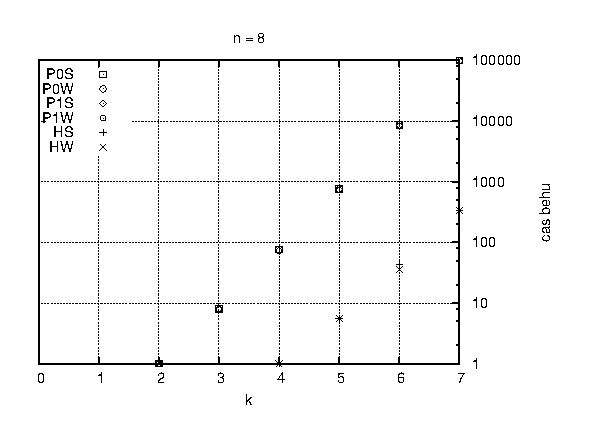
\includegraphics{graph/n8kid-cas}}
\caption{Průměrné časy běhů řešičů na 16 náhodných Rabinových hrách pro $n = 8$}
\label{fig:n8kidcas}
\end{figure}
V~grafu \ref{fig:n8kidcas} jsou zachyceny časy běhů řešičů nad hrami pro fixní $n = 8$ a $k$ pokrývající interval od $0$ do $7$. Pro každé $k$ bylo vygenerováno 16 náhodných her. Vynesené časy běhů jsou průměry přes tyto šestnáctice. Naměřené časy běhů jsou vyneseny v~logaritmické škále.

Fixní $n = 8$ jsem vybral experimentálně jako dostatečně velké pro \uv{zajímavé} chování vzhledem ke $k$.

V~grafu jde vidět, že na použitých hodnotách $n$ a $k$ se jednotlivé varianty Pitermanova řešiče a jednotlivé varianty Hornova řešiče výkonem téměř neliší.\footnote{Jednotlivé varianty řešičů jsou si výsledky tak podobné, že v~grafu téměř splývají. Shluky bodů vynesené výše na ose času běhu patří Pitermanovým řešičům a shluky bodů vynesené níže patří Hornovým řešičům.}

Dále lze pozorovat, že Hornovy řešiče mají proti Pitermanovým výrazně lepší časy běhů.

Absenci hodnot v~levé části grafu přisuzuji nízké rozlišovací schopnosti použitého systému pro měření času -- pro $k \leq 1$ byl na všech řešičích a pro $k \leq 3$ na Hornových řešičích naměřen nulový čas.
\subsubsection{Časy řešení pro $k = 4$}
\begin{figure}[htbp]
\centering
\resizebox{\textwidth}{!}{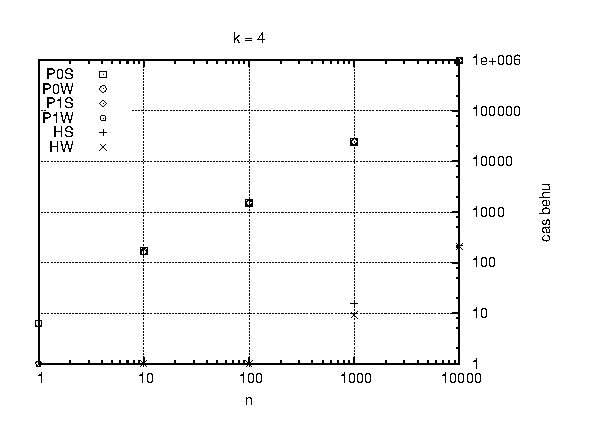
\includegraphics{graph/k4nexp-cas}}
\caption{Průměrné časy běhů řešičů na 16 náhodných Rabinových hrách pro $k = 4$}
\label{fig:k4nexp}
\end{figure}
V~grafu \ref{fig:k4nexp} jsou zachyceny časy běhů řešičů nad hrami pro fixní $k = 4$ a $n$ pokrývající interval od $1$ do $10000$ v~exponenciálních skocích (o základu $10$). Pro každé $n$ bylo vygenerováno 16 náhodných her. Vynesené časy běhů jsou průměry přes tyto šestnáctice. $n$ a naměřené časy běhů jsou vynesené v~logaritmických škálách.

Fixní $k = 4$ jsem vybral experimentálně jako dostatečně velké pro \uv{zajímavé} chování vzhledem k~$n$.

Graf naznačuje podobné relativní vlastnosti řešičů, jako graf \ref{fig:n8kidcas}, zejména podobnost jednotlivých variant řešiců a výrazný rozestup výkonu řešičů ve prospěch Hornova.

Dalo se očekávat, že čas řešení bude velmi podobný pro plné a částečné řešení, protože řešení strategie v~žádném z~použitých algoritmů nezvyšuje asymptotickou složitost. Tento předpoklad analýza potvrdila. Pro další testy jsem se proto rozhodl používat pouze ty varianty řešičů, které řeší plné řešení.

Překvapivým výsledkem je poměrně špatný výkon store-op\-ti\-ma\-li\-zo\-va\-né\-ho Pitermanova řešiče vzhledem k~Pitermanovu řešiči bez optimalizace. Zejména se nezdá, že by vykazoval asymptoticky menší časovou náročnost. Zůstává otázkou, jestli je tato podobnost zapříčiněna neefektivní implementací nebo výběrem testovacích her.
\chapter{Závěr} \label{chap:conclusions}
Úspěšně jsem implementoval algoritmy pro řešení Rabinových her představené v~článcích \cite{Piterman2006} a \cite{Horn2005}. Pro tyto implementace jsem vytvořil uživatelské rozhraní ve formě aplikace \rgsexe{} pro operační systém Windows. Implementoval jsem rozhraní mezi touto aplikací a softwarem MATLAB, prostřednictvím kterého lze řešit Rabinovy hry pomocí řešiče implementovaného ve skriptovacím jazyce softwaru MATLAB. Vytvořil jsem aplikaci \benchexe, která umožňuje dávkové testování časové efektivity řešičů na náhodných hrách.

V~provedených testech se ukázal jako časově výrazně efektivnější Hornův řešič.

Asymptoticky paměťově značně náročná optimalizace Pitermanova algoritmu, která zaručuje výrazné snížení asymptotické časové složitosti, se v~praxi na rychlosti řešení testovacích her neprojevila.
\paragraph{}
Zajímavými možnostmi dalšího vývoje řešiče jsou rozšíření na Streettovy hry a paralelizace výpočtů.

Mohlo by být zajímavé porovnat Pitermanův a Hornův řešič s~MATLABovým řešičem speciálně na hrách, které splňují jeho vstupní podmínky, s~efektivní metodou převodu (bez nárůstu velikosti instance, viz \ref{sec:matlab:prevod:narustvelikostiinstance}).
\bibliographystyle{plain}
\bibliography{bachelor}
\printindex
\appendix
\chapter{Digitální příloha}
\section{Obsah}
V~tabulce \ref{tab:obsahdigitalniprilohy} najdete výčet adresářů a vybraných souborů digitální přílohy s~jejich popisy.
\begin{longtable}{l|l}
\caption{Obsah digitální přílohy} \label{tab:obsahdigitalniprilohy} \\
\multicolumn{1}{l|}{\textbf{Cesta}} & \multicolumn{1}{l}{\textbf{Význam}} \\ \hline 
\endfirsthead

\multicolumn{2}{c}%
{{\tablename\ \thetable{}}} \\
\multicolumn{1}{l|}{\textbf{Cesta}} &
\multicolumn{1}{l}{\textbf{Význam}} \\ \hline 
\endhead

\path{program} & Soubory programů \\
\path{program/matlab} & Skripty MATLABového řešiče \\
\path{program/matlab/*.m} & Skripty MATLABového řešiče \\
\path{program/matlab/b2-2-1.mat} & Soubor s~nesprávně řešenou hrou \\
\path{program/src} & Soubory programů \\
\path{program/src/bench} & Soubory programu \benchexe \\
\path{program/src/bench/*.hpp} & Hlavičkové soubory \\
\path{program/src/bench/*.cpp} & Zdrojové soubory \\
\path{program/src/bench/bench.exe} & \emph{Program \benchexe} \\
\path{program/src/main} & Soubory programu \rgsexe \\
\path{program/src/main/*.hpp} & Hlavičkové soubory \\
\path{program/src/main/*.cpp} & Zdrojové soubory \\
\path{program/src/main/rgs.exe} & \emph{Program \rgsexe} \\
\path{program/src/env\_local.bat} & Lokální konfigurační skript \\
\path{program/src/env\_user.bat} & Uživatelský konfigurační skript \\
\path{program/bench.bat} & \emph{Zástupce \benchexe{} bez MATLABu} \\
\path{program/bench\_m.bat} & \emph{Zástupce \benchexe{} s~MATLABem} \\
\path{program/build.bat} & \emph{Hlavní kompilační skript} \\
\path{program/rgs.bat} & \emph{Zástupce \rgsexe{} bez MATLABu} \\
\path{program/rgs\_m.bat} & \emph{Zástupce \rgsexe{} s~MATLABem} \\
\path{text} & Soubory textu práce \\
\path{text/graph} & Zdrojové soubory grafů \\
\path{text/graph/*.dat} & Tabulky s~daty z~experimentů \\
\path{text/graph/*.plt} & Skripty pro generování grafů \\
\path{text/tex} & Dílčí zdrojové soubory \\
\path{text/tex/*.tex} & Dílčí zdrojové soubory \\
\path{text/bachelor.bib} & Zdrojový soubor bibliografie \\
\path{text/bachelor.pdf} & \emph{Text práce} \\
\path{text/bachelor.tex} & Hlavní zdrojový soubor textu práce \\
\path{text/bachelor.sty} & Zdrojový soubor stylu \\
\path{text/fi-logo.mf} & Logo Fakulty informatiky \\
\path{text/fit12.clo} & Dílčí soubor stylu fithesis2 \\
\path{text/fithesis2.cls} & Styl fithesis2 pro sazbu \\
\path{text/rgs.pdf} & \emph{Příručka programu \rgsexe} \\
\path{text/rgs.tex} & Zdrojový soubor příručky \rgsexe \\
\path{readme.txt} & Nápověda k~digitální příloze \\
\end{longtable}
\section{Nápověda}
Nápovědu k~programu \rgsexe{} najdete v~kapitole \ref{chap:rgsmanual}.

Nápovědu k~programu \benchexe{} získáte zavoláním programu \benchexe{} s~parametrem \path{-H} nebo \path{---help}.

Programy \rgsexe{} a \benchexe{} jsou ve verzi dodané v~digitální příloze sestavené bez MATLABového řešiče, aby byly kompatibilní s~více systémy. Pokud chcete používat MATLABový řešič, konzultujte sekci \ref{sec:rgsmanual:instalace}.
% Using fithesis2 LaTeX style.
% Required files: fithesis2.cls, fit12.clo, fi-logo.mf

% fithesis2 home page:
% http://is.muni.cz/th/173173/fi_b/?info

% fithesis2 documentation:
% http://is.muni.cz/th/173173/fi_b/thesis.pdf?info

% fithesis2 download:
% http://is.muni.cz/th/173173/fi_b/fithesis2.zip?info

%\documentclass[draft]{fithesis2} % Default: [12pt,oneside,onecolumn,final]
\documentclass{fithesis2} % Default: [12pt,oneside,onecolumn,final]
\usepackage{bachelor}
%%%
%% This is file `fithesis2.cls',
%% it's a software fork based on class fithesis v0.2.11 available
%% to download from http://www.fi.muni.cz/~xpavlov/fithesis/
%% This file is distributed under LPPL Version 1.3c

\NeedsTeXFormat{LaTeX2e}
\ProvidesClass{fithesis2}[2008/12/15 version 0.1 MU thesis class]

\ifx\clsclass\undefined
 \def\clsclass{rapport3}
\fi
\LoadClass{\clsclass}

% Declaration of documentclass options 
\DeclareOption{10pt}{\renewcommand\@ptsize{0}}
\DeclareOption{11pt}{\renewcommand\@ptsize{1}}
\DeclareOption{12pt}{\renewcommand\@ptsize{2}}
\DeclareOption{oneside}{\@twosidefalse \@mparswitchfalse}
\DeclareOption{twoside}{\@twosidetrue  \@mparswitchtrue}
\DeclareOption{onecolumn}{\@twolumnfalse}
\DeclareOption{twocolumn}{\@twocolumntrue}
\DeclareOption{draft}{\setlength\overfullrule{5pt}}
\DeclareOption{final}{\setlength\overfullrule{0pt}}

% Options executed by default
\ExecuteOptions{12pt,oneside,final}
\ProcessOptions

\RequirePackage{palatino}

\def\Scrreprtcls{scrreprt}
\def\Rapport1cls{rapport1}
\def\Rapport3cls{rapport3}

\ifx\clsclass\Scrreprtcls
 \newcommand*\ChapFont{\bfseries}
 \newcommand*\PageFont{\bfseries}
\fi

% depth of table of content (TOC)
% TOC will contain sectioning commands upto \subsubsection
\setcounter{tocdepth}{4}

% loads fit1*.clo size option class
\input fit1\@ptsize.clo\relax

\def\ps@thesisheadings{%
\def\chaptermark##1{%
\markright{%
\ifnum\c@secnumdepth >\m@ne
\thechapter.\ %
\fi ##1}}
\let\@oddfoot\@empty
\let\@oddhead\@empty
\def\@oddhead{\vbox{\hbox to \textwidth{%
\hfil{\sc\rightmark}}\vskip 4pt\hrule}}
\if@twoside
 \def\@evenhead{\vbox{\hbox to \textwidth{%
 {\sc\rightmark}\hfil}\vskip 4pt\hrule}}
\else
 \let\@evenhead\@oddhead
\fi
\def\@oddfoot{\hfil\PageFont\thepage}
\if@twoside
 \def\@evenfoot{\PageFont\thepage\hfil}%
\else
 \let\@evenfoot\@oddfoot
\fi
}

% defines style of the chapter heading
\renewcommand*\chapter{%
\if@twoside
 \clearpage
 \thispagestyle{empty}
 \cleardoublepage
\else
 \clearpage
\fi
\thispagestyle{plain}%
\global\@topnum\z@
\@afterindentfalse
\secdef\@chapter\@schapter}

% defines style of part heading
\renewcommand*\part{%
\clearpage
\thispagestyle{empty}
\cleardoublepage
\thispagestyle{empty}%
\if@twocolumn%
 \onecolumn
 \@tempswatrue
\else
 \@tempswafalse
\fi
\hbox{}\vfil
\secdef\@part\@spart}

% defines commands to typeset logos and default names of university,
% faculty and thesis title on the title page
\font\filogo fi-logo at 40mm % as logo of FI, METAFONT logo will be used
\def\facultylogo{\@thesisfaculty-logo} % log format
\def\universityname{Masarykova univerzita} % default university name
\def\facultyname{Fakulta informatiky} % default faculty name
\def\@thesissubtitle{Diplomov\'{a} pr\'{a}ce} % default thesis title
\def\lowecasewrapper#1{\lowercase{#1}}

% definition of \thesisfaculty options 
\def\Fi{fi} % Faculty of Informatics
\def\Sci{sci} % Faculty of Science
\def\Law{law} % Faculty of Law
\def\Eco{eco} % Faculty of Economics and Administration
\def\Fss{fss} % Faculty of Social studies
\def\Med{med} % Faculty of Medicine
\def\Ped{ped} % Faculty of Education
\def\Phil{phil} % Faculty of Arts
\def\Fsps{fsps} % Faculty of Sport Studies
\def\True{true}

% definition of language support: Czech (default), English and Slovak
\def\Langcs{cs}
\def\Langsk{sk}
\def\Langen{en}
\def\@thesislang{cs}

% definition of commands that will be used to typeset title page
% can be redefined in the source document
\def\titlefont{\fontsize\@xxvpt{30}\selectfont} 
\def\thesistitle#1{\gdef\@thesistitle{#1}}
\def\thesisstudent#1{\gdef\@thesisstudent{#1}}
\def\thesisyear#1{\gdef\@thesisyear{#1}}
\def\thesisplaceyear{Brno, \@thesisyear}
\def\thesissubtitle#1{\gdef\@thesissubtitle{#1}}
\def\thesisuniversity#1{\gdef\@thesisuniversity{#1}}
\def\thesislogo#1{\gdef\@thesislogo{#1}}
\def\thesisadvisor#1{\gdef\@thesisadvisor{#1}}
% option of \thesisfaculty macro defines which name of faculty will be printed
% language option defines whether english or czech name will be used
\def\thesisfaculty#1{\gdef\@thesisfaculty{#1}
\ifx\@thesisfaculty\Fi
 \ifx\@thesislang\Langen
  \def\facultyname{Faculty of Informatics}
  \def\universityname{Masaryk University}
   \else \def\facultyname{Fakulta informatiky}
  \fi
 \else \ifx\@thesisfaculty\Sci
  \ifx\@thesislang\Langen
   \def\facultyname{Faculty of Science}
   \def\universityname{Masaryk University}
  \else \def\facultyname{P\v{r}\'{i}rodov\v{e}deck\'{a} fakulta}
  \fi
  \else \ifx\@thesisfaculty\Law
   \ifx\@thesislang\Langen
    \def\facultyname{Faculty of Law}
    \def\universityname{Masaryk University}
   \else \def\facultyname{Pr\'{a}vnick\'{a} fakulta}
   \fi
  \else \ifx\@thesisfaculty\Eco
   \ifx\@thesislang\Langen
    \def\facultyname{Faculty of Economics and Administration}
    \def\universityname{Masaryk University}
   \else \def\facultyname{Ekonomicko-spr\'{a}vn\'{i} fakulta}
   \fi
  \else \ifx\@thesisfaculty\Fss
   \ifx\@thesislang\Langen
    \def\facultyname{Faculty of Social Studies}
    \def\universityname{Masaryk University}
   \else \def\facultyname{Fakulta soci\'{a}ln\'{i}ch studi\'{i}}
   \fi
  \else \ifx\@thesisfaculty\Med
   \ifx\@thesislang\Langen
    \def\facultyname{Faculty of Medicine}
    \def\universityname{Masaryk University}
   \else \def\facultyname{L\'{e}ka\v{r}sk\'{a} fakulta}
   \fi
  \else \ifx\@thesisfaculty\Ped
   \ifx\@thesislang\Langen
    \def\facultyname{Faculty of Education}
    \def\universityname{Masaryk University}
   \else \def\facultyname{Pedagogick\'{a} fakulta}
   \fi
  \else \ifx\@thesisfaculty\Phil
   \ifx\@thesislang\Langen
    \def\facultyname{Faculty of Arts}
    \def\universityname{Masaryk University}
   \else \def\facultyname{Filozofick\'{a} fakulta}
   \fi
  \else \ifx\@thesisfaculty\Fsps
   \ifx\@thesislang\Langen
    \def\facultyname{Faculty of Sports Studies}
    \def\universityname{Masaryk University}
   \else \def\facultyname{Fakulta sportovn\'{i}ch studi\'{i}}
   \fi
         \else
          \def\facultyname{\@thesisfaculty}
          \def\universityname{\@thesisuniversity}
          \def\facultylogo{\@thesislogo}
          \def\thesisplaceyear{\@thesisyear}
         \fi
        \fi
       \fi
      \fi
     \fi
    \fi
   \fi
  \fi
\fi
}

\newif\if@restonecol

\def\alwayssingle{%
\@restonecolfalse\if@twocolumn\@restonecoltrue\onecolumn\fi}
\def\endalwayssingle{\if@restonecol\twocolumn\fi}

% if the true value is set in the \thesiswoman command
% then character 'a' will be added after verbs in czech and
% slovak language when typesetting declaration text
\newif\ifwoman\womanfalse
\def\@w{\ifwoman{a}\else\fi}
\def\thesiswoman#1{\gdef\@thesiswoman{#1}
\ifx\@thesiswoman\True\def\@w{a}\else\def\@w{}\fi}

\def\thesislang#1{\gdef\@thesislang{#1}}

% Text of Declaration in Czech
\def\DeclarationTextcs{%
Prohla\v{s}uji, \v{z}e tato \expandafter\lowecasewrapper\@thesissubtitle{}
je m\'{y}m p\r{u}vodn\'{i}m autorsk\'{y}m
d\'{i}lem, kter\'{e} jsem vypracoval\@w\ samostatn\v{e}. V\v{s}echny zdroje, prameny a
literaturu, kter\'{e} jsem p\v{r}i vypracov\'{a}n\'{i} pou\v{z}\'{i}val\@w\ nebo z~nich
\v{c}erpal\@w, v~pr\'{a}ci \v{r}\'{a}dn\v{e} cituji s~uveden\'{i}m \'{u}pln\'{e}ho odkazu na p\v{r}\'{i}slu\v{s}n\'{y}
zdroj.}
% in Slovak
\def\DeclarationTextsk{%
Prehlasujem, \v{z}e t\'{a}to \expandafter\lowecasewrapper\@thesissubtitle{}
je moj\'{i}m p\^{o}vodn\'{y}m autorsk\'{y}m
dielom, ktor\'{e} som vypracoval\@w\ samostatne. V\v{s}etky zdroje, pramene a
literat\'{u}ru, ktor\'{e} som pri vypracovan\'{i} pou\v{z}\'{i}val\@w\ alebo z~nich
\v{c}erpal\@w, v~pr\'{a}ci riadne citujem s~uveden\'{i}m \'{u}pln\'{e}ho odkazu na pr\'{i}slu\v{s}n\'{y}
zdroj.}
% in English
\def\DeclarationTexten{%
Hereby I declare, that this paper is my original authorial work,
which I have worked out by my own. All sources, references and literature used or excerpted
during elaboration of this work are properly cited and listed in complete reference to the due source.
}

% Declaration heading in Czech
\def\DeclarationTitlecs{%
Prohl\'{a}\v{s}en\'{i}
}
% in Slovak
\def\DeclarationTitlesk{%
Prehl\'{a}senie
}
% in English
\def\DeclarationTitleen{%
Declaration
}
% Heading of thesis thank
\def\ThanksTitlecs{%
Pod\v{e}kov\'{a}n\'{i}
}

\def\ThanksTitlesk{%
Po\v{d}akovanie
}

\def\ThanksTitleen{%
Acknowledgement
}
% definition of heading of thesis abstract
\def\AbstractTitlecs{%
Shrnut\'{i}
}

\def\AbstractTitlesk{%
Zhrnutie
}

\def\AbstractTitleen{%
Abstract
}

% definiton of heding of thesis Keywords
\def\KeyWordsTitlecs{%
Kl\'{i}\v{c}ov\'{a} slova
}

\def\KeyWordsTitlesk{%
K\v{l}\'{u}\v{c}ov\'{e} slov\'{a}
}

\def\KeyWordsTitleen{%
Keywords
}
% Definition of command used to declare thesis advisor heading
\def\AdvisorTitlecs{%
Vedouc\'{i} pr\'{a}ce:
}

\def\AdvisorTitlesk{%
Ved\'{u}ci pr\'{a}ce:
}

\def\AdvisorTitleen{%
Advisor:
}

% command prints declaration text in defined language
% with name of student under it
\def\DeclarationText{%
\ifx\@thesislang\Langcs
 \DeclarationTextcs
 \else \ifx\@thesislang\Langsk
  \DeclarationTextsk
  \else \ifx\@thesislang\Langen
   \DeclarationTexten
   \else \DeclarationTextcs
  \fi
 \fi
\fi
\vskip 2cm
\hfill\@thesisstudent
}
% prints "Advisor:" in defined language
\def\AdvisorName{\par\vfill{
\ifx\@thesislang\Langcs
 \bf \AdvisorTitlecs
 \else \ifx\@thesislang\Langsk
  \bf \AdvisorTitlesk
  \else \ifx\@thesislang\Langen
   \bf \AdvisorTitleen
   \else \bf \AdvisorTitlecs
  \fi
 \fi
\fi} \@thesisadvisor}

% this command begins compulsory part of the thesis
% page numbering will be roman
\def\FrontMatter{%
\pagestyle{plain}
\parindent 1.5em
\setcounter{page}{1}
\pagenumbering{roman}}

% command to typeset thesis title page
\newcommand{\ThesisTitlePage}{
\begin{alwayssingle}
\thispagestyle{empty}
\begin{center}
{\sc \universityname\\ \facultyname}
\vskip 1em

% if FI then logo in METAFONT format will be typeset
\ifx\@thesisfaculty\Fi
 {\filogo SL}\\[0.4in]
% else logo defined in \facultylogo command will be used
\else
 \includegraphics[width=40mm]{\facultylogo}\\[0.4in]
\fi

% typesets thesis subtitle and the name of author
% with year and place of university
\let\footnotesize\small
\let\footnoterule\relax{}
{\titlefont\bf\@thesistitle\par\vfil}\vskip 0.8in
{\sc \@thesissubtitle}\\[0.3in]
{\Large\bf\@thesisstudent}
\par\vfill
{\large \thesisplaceyear}
\end{center}
\end{alwayssingle}
\newpage}

% definition of new environment that will print thesis
% declaration in specified language
\newenvironment{ThesisDeclaration}{%
\begin{alwayssingle}
\ifx\@thesislang\Langcs
 \chapter*{\DeclarationTitlecs}
 \else \ifx\@thesislang\Langsk
  \chapter*{\DeclarationTitlesk}
  \else \ifx\@thesislang\Langen
   \chapter*{\DeclarationTitleen}
   \else \chapter*{\DeclarationTitlecs}
  \fi
 \fi
\fi}
{\par\vfil
\end{alwayssingle}
\newpage}

% new environment that typesets thesis thank
\newenvironment{ThesisThanks}{%
\begin{alwayssingle}
\ifx\@thesislang\Langcs
 \chapter*{\ThanksTitlecs}
 \else \ifx\@thesislang\Langsk
  \chapter*{\ThanksTitlesk}
  \else \ifx\@thesislang\Langen
   \chapter*{\ThanksTitleen}
   \else \chapter*{\ThanksTitlecs}
  \fi
 \fi
\fi}
{\par\vfill
\end{alwayssingle}
\newpage}

% typesets thesis abstract
\newenvironment{ThesisAbstract}{%
\begin{alwayssingle}
\ifx\@thesislang\Langcs
 \chapter*{\AbstractTitlecs}
 \else \ifx\@thesislang\Langsk
  \chapter*{\AbstractTitlesk}
  \else \ifx\@thesislang\Langen
   \chapter*{\AbstractTitleen}
   \else \chapter*{\AbstractTitlecs}
  \fi
 \fi
\fi}
{\par\vfil\null
\end{alwayssingle}
\newpage}

% typesets thesis abstract in English
% not used in fithesis2
%\newenvironment{ThesisAbstracten}{%
%\begin{alwayssingle}
%\chapter*{\AbstractTitleen}
%}
%{\par\vfil\null
%\end{alwayssingle}
%\newpage}

% typesets thesis keywords 
\newenvironment{ThesisKeyWords}{%
\begin{alwayssingle}
\ifx\@thesislang\Langcs
 \chapter*{\KeyWordsTitlecs}
 \else \ifx\@thesislang\Langsk
  \chapter*{\KeyWordsTitlesk}
  \else \ifx\@thesislang\Langen
   \chapter*{\KeyWordsTitleen}
   \else \chapter*{\KeyWordsTitlecs}
  \fi
 \fi
\fi}
{\par\vfill
\end{alwayssingle}
\newpage}

% defines MainMatter command that begins main part
% of the thesis with Arabic page numbering
\def\MainMatter{%
\if@twoside
 \clearpage
 \thispagestyle{empty}
 \cleardoublepage
\else
 \clearpage
\fi
\setcounter{page}{1}
\pagenumbering{arabic}
\pagestyle{thesisheadings}
\parindent 1.5em}


\renewcommand*\l@part[2]{%
  \ifnum \c@tocdepth >-2\relax
    \addpenalty{-\@highpenalty}%
    \addvspace{0.5em \@plus\p@}%
    \begingroup
      \setlength\@tempdima{3em}%
      \parindent \z@ \rightskip \@pnumwidth
      \parfillskip -\@pnumwidth
      {\leavevmode
       \normalfont \bfseries #1\hfil \hb@xt@\@pnumwidth{\hss #2}}\par
       \nobreak
         \global\@nobreaktrue
         \everypar{\global\@nobreakfalse\everypar{}}%
    \endgroup
    \addvspace{0.2em \@plus\p@}%
  \fi}

\renewcommand*\l@chapter[2]{%
  \ifnum \c@tocdepth >\m@ne
    \addpenalty{-\@highpenalty}%
    \vskip 1.0em \@plus\p@
    \setlength\@tempdima{1.5em}%
    \begingroup
      \parindent \z@ \rightskip \@pnumwidth
      \parfillskip -\@pnumwidth
      \leavevmode \bfseries
      \advance\leftskip\@tempdima
      \hskip -\leftskip
      #1\nobreak\hfil \nobreak\hb@xt@\@pnumwidth{\hss #2}\par
      \penalty\@highpenalty
    \endgroup
  \fi}

\renewcommand*\l@chapter{\@dottedtocline{1}{0em}{1.5em}}
\renewcommand*\l@section{\@dottedtocline{2}{1.5em}{2.3em}}
\renewcommand*\l@subsection{\@dottedtocline{2}{3.8em}{3.2em}}
\renewcommand*\l@subsubsection{\@dottedtocline{2}{7.0em}{3.8em}}

\endinput
%%
%% End of file `fithesis2.cls'.


% thesis.pdf:
% The hyperref package should be the very last line before \begin{document}
\usepackage[plainpages=false,pdfpagelabels,unicode]{hyperref}
%\usepackage{hyperref}
\begin{document}
% Using fithesis2 LaTeX style.
% Required files: fithesis2.cls, fit12.clo, fi-logo.mf

% fithesis2 home page:
% http://is.muni.cz/th/173173/fi_b/?info

% fithesis2 documentation:
% http://is.muni.cz/th/173173/fi_b/thesis.pdf?info

% fithesis2 download:
% http://is.muni.cz/th/173173/fi_b/fithesis2.zip?info

%\documentclass[draft]{fithesis2} % Default: [12pt,oneside,onecolumn,final]
\documentclass{fithesis2} % Default: [12pt,oneside,onecolumn,final]
\usepackage{bachelor}
%%%
%% This is file `fithesis2.cls',
%% it's a software fork based on class fithesis v0.2.11 available
%% to download from http://www.fi.muni.cz/~xpavlov/fithesis/
%% This file is distributed under LPPL Version 1.3c

\NeedsTeXFormat{LaTeX2e}
\ProvidesClass{fithesis2}[2008/12/15 version 0.1 MU thesis class]

\ifx\clsclass\undefined
 \def\clsclass{rapport3}
\fi
\LoadClass{\clsclass}

% Declaration of documentclass options 
\DeclareOption{10pt}{\renewcommand\@ptsize{0}}
\DeclareOption{11pt}{\renewcommand\@ptsize{1}}
\DeclareOption{12pt}{\renewcommand\@ptsize{2}}
\DeclareOption{oneside}{\@twosidefalse \@mparswitchfalse}
\DeclareOption{twoside}{\@twosidetrue  \@mparswitchtrue}
\DeclareOption{onecolumn}{\@twolumnfalse}
\DeclareOption{twocolumn}{\@twocolumntrue}
\DeclareOption{draft}{\setlength\overfullrule{5pt}}
\DeclareOption{final}{\setlength\overfullrule{0pt}}

% Options executed by default
\ExecuteOptions{12pt,oneside,final}
\ProcessOptions

\RequirePackage{palatino}

\def\Scrreprtcls{scrreprt}
\def\Rapport1cls{rapport1}
\def\Rapport3cls{rapport3}

\ifx\clsclass\Scrreprtcls
 \newcommand*\ChapFont{\bfseries}
 \newcommand*\PageFont{\bfseries}
\fi

% depth of table of content (TOC)
% TOC will contain sectioning commands upto \subsubsection
\setcounter{tocdepth}{4}

% loads fit1*.clo size option class
\input fit1\@ptsize.clo\relax

\def\ps@thesisheadings{%
\def\chaptermark##1{%
\markright{%
\ifnum\c@secnumdepth >\m@ne
\thechapter.\ %
\fi ##1}}
\let\@oddfoot\@empty
\let\@oddhead\@empty
\def\@oddhead{\vbox{\hbox to \textwidth{%
\hfil{\sc\rightmark}}\vskip 4pt\hrule}}
\if@twoside
 \def\@evenhead{\vbox{\hbox to \textwidth{%
 {\sc\rightmark}\hfil}\vskip 4pt\hrule}}
\else
 \let\@evenhead\@oddhead
\fi
\def\@oddfoot{\hfil\PageFont\thepage}
\if@twoside
 \def\@evenfoot{\PageFont\thepage\hfil}%
\else
 \let\@evenfoot\@oddfoot
\fi
}

% defines style of the chapter heading
\renewcommand*\chapter{%
\if@twoside
 \clearpage
 \thispagestyle{empty}
 \cleardoublepage
\else
 \clearpage
\fi
\thispagestyle{plain}%
\global\@topnum\z@
\@afterindentfalse
\secdef\@chapter\@schapter}

% defines style of part heading
\renewcommand*\part{%
\clearpage
\thispagestyle{empty}
\cleardoublepage
\thispagestyle{empty}%
\if@twocolumn%
 \onecolumn
 \@tempswatrue
\else
 \@tempswafalse
\fi
\hbox{}\vfil
\secdef\@part\@spart}

% defines commands to typeset logos and default names of university,
% faculty and thesis title on the title page
\font\filogo fi-logo at 40mm % as logo of FI, METAFONT logo will be used
\def\facultylogo{\@thesisfaculty-logo} % log format
\def\universityname{Masarykova univerzita} % default university name
\def\facultyname{Fakulta informatiky} % default faculty name
\def\@thesissubtitle{Diplomov\'{a} pr\'{a}ce} % default thesis title
\def\lowecasewrapper#1{\lowercase{#1}}

% definition of \thesisfaculty options 
\def\Fi{fi} % Faculty of Informatics
\def\Sci{sci} % Faculty of Science
\def\Law{law} % Faculty of Law
\def\Eco{eco} % Faculty of Economics and Administration
\def\Fss{fss} % Faculty of Social studies
\def\Med{med} % Faculty of Medicine
\def\Ped{ped} % Faculty of Education
\def\Phil{phil} % Faculty of Arts
\def\Fsps{fsps} % Faculty of Sport Studies
\def\True{true}

% definition of language support: Czech (default), English and Slovak
\def\Langcs{cs}
\def\Langsk{sk}
\def\Langen{en}
\def\@thesislang{cs}

% definition of commands that will be used to typeset title page
% can be redefined in the source document
\def\titlefont{\fontsize\@xxvpt{30}\selectfont} 
\def\thesistitle#1{\gdef\@thesistitle{#1}}
\def\thesisstudent#1{\gdef\@thesisstudent{#1}}
\def\thesisyear#1{\gdef\@thesisyear{#1}}
\def\thesisplaceyear{Brno, \@thesisyear}
\def\thesissubtitle#1{\gdef\@thesissubtitle{#1}}
\def\thesisuniversity#1{\gdef\@thesisuniversity{#1}}
\def\thesislogo#1{\gdef\@thesislogo{#1}}
\def\thesisadvisor#1{\gdef\@thesisadvisor{#1}}
% option of \thesisfaculty macro defines which name of faculty will be printed
% language option defines whether english or czech name will be used
\def\thesisfaculty#1{\gdef\@thesisfaculty{#1}
\ifx\@thesisfaculty\Fi
 \ifx\@thesislang\Langen
  \def\facultyname{Faculty of Informatics}
  \def\universityname{Masaryk University}
   \else \def\facultyname{Fakulta informatiky}
  \fi
 \else \ifx\@thesisfaculty\Sci
  \ifx\@thesislang\Langen
   \def\facultyname{Faculty of Science}
   \def\universityname{Masaryk University}
  \else \def\facultyname{P\v{r}\'{i}rodov\v{e}deck\'{a} fakulta}
  \fi
  \else \ifx\@thesisfaculty\Law
   \ifx\@thesislang\Langen
    \def\facultyname{Faculty of Law}
    \def\universityname{Masaryk University}
   \else \def\facultyname{Pr\'{a}vnick\'{a} fakulta}
   \fi
  \else \ifx\@thesisfaculty\Eco
   \ifx\@thesislang\Langen
    \def\facultyname{Faculty of Economics and Administration}
    \def\universityname{Masaryk University}
   \else \def\facultyname{Ekonomicko-spr\'{a}vn\'{i} fakulta}
   \fi
  \else \ifx\@thesisfaculty\Fss
   \ifx\@thesislang\Langen
    \def\facultyname{Faculty of Social Studies}
    \def\universityname{Masaryk University}
   \else \def\facultyname{Fakulta soci\'{a}ln\'{i}ch studi\'{i}}
   \fi
  \else \ifx\@thesisfaculty\Med
   \ifx\@thesislang\Langen
    \def\facultyname{Faculty of Medicine}
    \def\universityname{Masaryk University}
   \else \def\facultyname{L\'{e}ka\v{r}sk\'{a} fakulta}
   \fi
  \else \ifx\@thesisfaculty\Ped
   \ifx\@thesislang\Langen
    \def\facultyname{Faculty of Education}
    \def\universityname{Masaryk University}
   \else \def\facultyname{Pedagogick\'{a} fakulta}
   \fi
  \else \ifx\@thesisfaculty\Phil
   \ifx\@thesislang\Langen
    \def\facultyname{Faculty of Arts}
    \def\universityname{Masaryk University}
   \else \def\facultyname{Filozofick\'{a} fakulta}
   \fi
  \else \ifx\@thesisfaculty\Fsps
   \ifx\@thesislang\Langen
    \def\facultyname{Faculty of Sports Studies}
    \def\universityname{Masaryk University}
   \else \def\facultyname{Fakulta sportovn\'{i}ch studi\'{i}}
   \fi
         \else
          \def\facultyname{\@thesisfaculty}
          \def\universityname{\@thesisuniversity}
          \def\facultylogo{\@thesislogo}
          \def\thesisplaceyear{\@thesisyear}
         \fi
        \fi
       \fi
      \fi
     \fi
    \fi
   \fi
  \fi
\fi
}

\newif\if@restonecol

\def\alwayssingle{%
\@restonecolfalse\if@twocolumn\@restonecoltrue\onecolumn\fi}
\def\endalwayssingle{\if@restonecol\twocolumn\fi}

% if the true value is set in the \thesiswoman command
% then character 'a' will be added after verbs in czech and
% slovak language when typesetting declaration text
\newif\ifwoman\womanfalse
\def\@w{\ifwoman{a}\else\fi}
\def\thesiswoman#1{\gdef\@thesiswoman{#1}
\ifx\@thesiswoman\True\def\@w{a}\else\def\@w{}\fi}

\def\thesislang#1{\gdef\@thesislang{#1}}

% Text of Declaration in Czech
\def\DeclarationTextcs{%
Prohla\v{s}uji, \v{z}e tato \expandafter\lowecasewrapper\@thesissubtitle{}
je m\'{y}m p\r{u}vodn\'{i}m autorsk\'{y}m
d\'{i}lem, kter\'{e} jsem vypracoval\@w\ samostatn\v{e}. V\v{s}echny zdroje, prameny a
literaturu, kter\'{e} jsem p\v{r}i vypracov\'{a}n\'{i} pou\v{z}\'{i}val\@w\ nebo z~nich
\v{c}erpal\@w, v~pr\'{a}ci \v{r}\'{a}dn\v{e} cituji s~uveden\'{i}m \'{u}pln\'{e}ho odkazu na p\v{r}\'{i}slu\v{s}n\'{y}
zdroj.}
% in Slovak
\def\DeclarationTextsk{%
Prehlasujem, \v{z}e t\'{a}to \expandafter\lowecasewrapper\@thesissubtitle{}
je moj\'{i}m p\^{o}vodn\'{y}m autorsk\'{y}m
dielom, ktor\'{e} som vypracoval\@w\ samostatne. V\v{s}etky zdroje, pramene a
literat\'{u}ru, ktor\'{e} som pri vypracovan\'{i} pou\v{z}\'{i}val\@w\ alebo z~nich
\v{c}erpal\@w, v~pr\'{a}ci riadne citujem s~uveden\'{i}m \'{u}pln\'{e}ho odkazu na pr\'{i}slu\v{s}n\'{y}
zdroj.}
% in English
\def\DeclarationTexten{%
Hereby I declare, that this paper is my original authorial work,
which I have worked out by my own. All sources, references and literature used or excerpted
during elaboration of this work are properly cited and listed in complete reference to the due source.
}

% Declaration heading in Czech
\def\DeclarationTitlecs{%
Prohl\'{a}\v{s}en\'{i}
}
% in Slovak
\def\DeclarationTitlesk{%
Prehl\'{a}senie
}
% in English
\def\DeclarationTitleen{%
Declaration
}
% Heading of thesis thank
\def\ThanksTitlecs{%
Pod\v{e}kov\'{a}n\'{i}
}

\def\ThanksTitlesk{%
Po\v{d}akovanie
}

\def\ThanksTitleen{%
Acknowledgement
}
% definition of heading of thesis abstract
\def\AbstractTitlecs{%
Shrnut\'{i}
}

\def\AbstractTitlesk{%
Zhrnutie
}

\def\AbstractTitleen{%
Abstract
}

% definiton of heding of thesis Keywords
\def\KeyWordsTitlecs{%
Kl\'{i}\v{c}ov\'{a} slova
}

\def\KeyWordsTitlesk{%
K\v{l}\'{u}\v{c}ov\'{e} slov\'{a}
}

\def\KeyWordsTitleen{%
Keywords
}
% Definition of command used to declare thesis advisor heading
\def\AdvisorTitlecs{%
Vedouc\'{i} pr\'{a}ce:
}

\def\AdvisorTitlesk{%
Ved\'{u}ci pr\'{a}ce:
}

\def\AdvisorTitleen{%
Advisor:
}

% command prints declaration text in defined language
% with name of student under it
\def\DeclarationText{%
\ifx\@thesislang\Langcs
 \DeclarationTextcs
 \else \ifx\@thesislang\Langsk
  \DeclarationTextsk
  \else \ifx\@thesislang\Langen
   \DeclarationTexten
   \else \DeclarationTextcs
  \fi
 \fi
\fi
\vskip 2cm
\hfill\@thesisstudent
}
% prints "Advisor:" in defined language
\def\AdvisorName{\par\vfill{
\ifx\@thesislang\Langcs
 \bf \AdvisorTitlecs
 \else \ifx\@thesislang\Langsk
  \bf \AdvisorTitlesk
  \else \ifx\@thesislang\Langen
   \bf \AdvisorTitleen
   \else \bf \AdvisorTitlecs
  \fi
 \fi
\fi} \@thesisadvisor}

% this command begins compulsory part of the thesis
% page numbering will be roman
\def\FrontMatter{%
\pagestyle{plain}
\parindent 1.5em
\setcounter{page}{1}
\pagenumbering{roman}}

% command to typeset thesis title page
\newcommand{\ThesisTitlePage}{
\begin{alwayssingle}
\thispagestyle{empty}
\begin{center}
{\sc \universityname\\ \facultyname}
\vskip 1em

% if FI then logo in METAFONT format will be typeset
\ifx\@thesisfaculty\Fi
 {\filogo SL}\\[0.4in]
% else logo defined in \facultylogo command will be used
\else
 \includegraphics[width=40mm]{\facultylogo}\\[0.4in]
\fi

% typesets thesis subtitle and the name of author
% with year and place of university
\let\footnotesize\small
\let\footnoterule\relax{}
{\titlefont\bf\@thesistitle\par\vfil}\vskip 0.8in
{\sc \@thesissubtitle}\\[0.3in]
{\Large\bf\@thesisstudent}
\par\vfill
{\large \thesisplaceyear}
\end{center}
\end{alwayssingle}
\newpage}

% definition of new environment that will print thesis
% declaration in specified language
\newenvironment{ThesisDeclaration}{%
\begin{alwayssingle}
\ifx\@thesislang\Langcs
 \chapter*{\DeclarationTitlecs}
 \else \ifx\@thesislang\Langsk
  \chapter*{\DeclarationTitlesk}
  \else \ifx\@thesislang\Langen
   \chapter*{\DeclarationTitleen}
   \else \chapter*{\DeclarationTitlecs}
  \fi
 \fi
\fi}
{\par\vfil
\end{alwayssingle}
\newpage}

% new environment that typesets thesis thank
\newenvironment{ThesisThanks}{%
\begin{alwayssingle}
\ifx\@thesislang\Langcs
 \chapter*{\ThanksTitlecs}
 \else \ifx\@thesislang\Langsk
  \chapter*{\ThanksTitlesk}
  \else \ifx\@thesislang\Langen
   \chapter*{\ThanksTitleen}
   \else \chapter*{\ThanksTitlecs}
  \fi
 \fi
\fi}
{\par\vfill
\end{alwayssingle}
\newpage}

% typesets thesis abstract
\newenvironment{ThesisAbstract}{%
\begin{alwayssingle}
\ifx\@thesislang\Langcs
 \chapter*{\AbstractTitlecs}
 \else \ifx\@thesislang\Langsk
  \chapter*{\AbstractTitlesk}
  \else \ifx\@thesislang\Langen
   \chapter*{\AbstractTitleen}
   \else \chapter*{\AbstractTitlecs}
  \fi
 \fi
\fi}
{\par\vfil\null
\end{alwayssingle}
\newpage}

% typesets thesis abstract in English
% not used in fithesis2
%\newenvironment{ThesisAbstracten}{%
%\begin{alwayssingle}
%\chapter*{\AbstractTitleen}
%}
%{\par\vfil\null
%\end{alwayssingle}
%\newpage}

% typesets thesis keywords 
\newenvironment{ThesisKeyWords}{%
\begin{alwayssingle}
\ifx\@thesislang\Langcs
 \chapter*{\KeyWordsTitlecs}
 \else \ifx\@thesislang\Langsk
  \chapter*{\KeyWordsTitlesk}
  \else \ifx\@thesislang\Langen
   \chapter*{\KeyWordsTitleen}
   \else \chapter*{\KeyWordsTitlecs}
  \fi
 \fi
\fi}
{\par\vfill
\end{alwayssingle}
\newpage}

% defines MainMatter command that begins main part
% of the thesis with Arabic page numbering
\def\MainMatter{%
\if@twoside
 \clearpage
 \thispagestyle{empty}
 \cleardoublepage
\else
 \clearpage
\fi
\setcounter{page}{1}
\pagenumbering{arabic}
\pagestyle{thesisheadings}
\parindent 1.5em}


\renewcommand*\l@part[2]{%
  \ifnum \c@tocdepth >-2\relax
    \addpenalty{-\@highpenalty}%
    \addvspace{0.5em \@plus\p@}%
    \begingroup
      \setlength\@tempdima{3em}%
      \parindent \z@ \rightskip \@pnumwidth
      \parfillskip -\@pnumwidth
      {\leavevmode
       \normalfont \bfseries #1\hfil \hb@xt@\@pnumwidth{\hss #2}}\par
       \nobreak
         \global\@nobreaktrue
         \everypar{\global\@nobreakfalse\everypar{}}%
    \endgroup
    \addvspace{0.2em \@plus\p@}%
  \fi}

\renewcommand*\l@chapter[2]{%
  \ifnum \c@tocdepth >\m@ne
    \addpenalty{-\@highpenalty}%
    \vskip 1.0em \@plus\p@
    \setlength\@tempdima{1.5em}%
    \begingroup
      \parindent \z@ \rightskip \@pnumwidth
      \parfillskip -\@pnumwidth
      \leavevmode \bfseries
      \advance\leftskip\@tempdima
      \hskip -\leftskip
      #1\nobreak\hfil \nobreak\hb@xt@\@pnumwidth{\hss #2}\par
      \penalty\@highpenalty
    \endgroup
  \fi}

\renewcommand*\l@chapter{\@dottedtocline{1}{0em}{1.5em}}
\renewcommand*\l@section{\@dottedtocline{2}{1.5em}{2.3em}}
\renewcommand*\l@subsection{\@dottedtocline{2}{3.8em}{3.2em}}
\renewcommand*\l@subsubsection{\@dottedtocline{2}{7.0em}{3.8em}}

\endinput
%%
%% End of file `fithesis2.cls'.


% thesis.pdf:
% The hyperref package should be the very last line before \begin{document}
\usepackage[plainpages=false,pdfpagelabels,unicode]{hyperref}
%\usepackage{hyperref}
\begin{document}
% Using fithesis2 LaTeX style.
% Required files: fithesis2.cls, fit12.clo, fi-logo.mf

% fithesis2 home page:
% http://is.muni.cz/th/173173/fi_b/?info

% fithesis2 documentation:
% http://is.muni.cz/th/173173/fi_b/thesis.pdf?info

% fithesis2 download:
% http://is.muni.cz/th/173173/fi_b/fithesis2.zip?info

%\documentclass[draft]{fithesis2} % Default: [12pt,oneside,onecolumn,final]
\documentclass{fithesis2} % Default: [12pt,oneside,onecolumn,final]
\usepackage{bachelor}
%\input{tex/fithesis2}

% thesis.pdf:
% The hyperref package should be the very last line before \begin{document}
\usepackage[plainpages=false,pdfpagelabels,unicode]{hyperref}
%\usepackage{hyperref}
\begin{document}
\input{tex/rgs.tex}
\end{document}
\end{document}
\end{document}
\end{document}